\renewcommand{\chaptername}{Software del microcontrolador}
\graphicspath{{parte_2/soft_micro/}}
\chapter{Software del Microcontrolador} 
%\markright{Software del microcontrolador}
\begin{center}
	\begin{tcolorbox}[colback=gray!5!white, %Color del fondo
		colframe=gray!75!black,
		title= \center{\Large{Resumen}} ]
		Se describe el proceso realizado para programar el software para el microcontrolador ATmega328P, bajo el entorno arduino, y sus librerías. Además, se muestra cómo deben interconectarse los componentes, y los circuitos correspondientes para realizar las pruebas sobre cada parte del software. Cada parte del software desarrollado, se realizan las verificaciones, y se muestran los resultados obtenidos. Una vez, realizadas todas las pruebas, se procede a integrar todo el software, y se realiza una prueba final, y se verifica la funcionalidad. La versión de software presentada en este capítulo, es una parte del desarrollo. En la siguiente fase del proyecto, se implementa e integra la parte restante del mismo (fase 3).   		 
 	\end{tcolorbox}
\end{center}    
\section{Introdución} 

	 El software, requiere del hardware seleccionado en el capítulo \ref{cap:cap3_sel_hw}. Este hardware, debe interconectarse entre sí antes de empezar a programarse sobre el microcontrolador. Una vez realizado este proceso, se desarrolla el software
	en base a los requerimientos de \ref{tab:requerimientos}. Para la programación, se divide el trabajo en el siguiente orden: 
	\begin{enumerate}
		\item Autocalibración: necesaria para que el software sea capaz de reconocer la orientación de la antena. 
		\item Control de posición: requiere que se realice la autocalibración correctamente. Esta función, decide los movimientos de giro de la antena en base a la autocalibración. 
		\item Scheduler o planificación: necesaria para realizar el control, a tiempo controlador, y no se utilice un esquema de polling.  
		\item Conexión del dispositivo a la red. Conectarse con Gpredict y stellarium: en esta parte del desarrollo, se realiza la programación de los protocolos implementados por cada uno de estos programas. Cada programa tiene protocolos distintos.
		\item Display LCD: se utiliza para mostrar información.  
	\end{enumerate}

%%	Una vez resueltos, todos los puntos anteriores, se pasa a unir todo el código desarrollado a lo largo de las presentes secciones de este capítulo. Luego, se deja comentado dentro del código aquellas partes que se desarrollen más adelante a lo largo de este texto. La parte que resta es la transformación de coordenadas, de coordenadas ecuatoriales a coordenadas locales horizontales.  El código en su versión final se muestra en el apéndice del documento. El código desarrollado hasta el momento, se presenta en el apéndice del presente capítulo.
%Estas funciones, que se mencionan, deben actuar sobre elementos de hardware. Estos, deben conectarse eléctricamente entre sí. Por este motivo, se empu
%En esta parte, se desarrolla la parte electrónica de los componentes de hardware como de software, empezando por los componentes de hardware y su interconexión. 

Luego del desarrollo de cada parte del software, se procede a su integración, y análisis del código, utilizando herramientas provistas por el fabricante del chip ATmega328P (microchip). 

\section{Diagrama del sistema} 

En base a los componentes seleccionados, en el capítulo \ref{cap:cap3_sel_hw}, estos deben interconectarse entre sí, mediante sus protocolos de comunicación. El sistema de control, se compone del diagrama en bloques mostrado en la figura \ref{fig:sistema_general}.  
\begin{figure}[ht]
	\hspace{-15mm}
%	\centering 
	\includegraphics{sistema_general} 
	\caption{Diagrama general del sistema de control} 
	\label{fig:sistema_general}
\end{figure}

Este diagrama en bloques muestra cual es el protocolo de comunicación utilizado por cada dispositivo. La conexión entre el bus SPI soportada por el microcontrolador y el chip ethernet, es el modo 0(ver apéndice \ref{AP:protSerial}), y la conexión con el display es mediante el protocolo I2C (descripto en el apéndice \ref{AP:protSerial}). El bloque de drivers de motores, son dos controladores de motores, y dos encoders, pero se ha puesto una único bloque, ya que el sistema de control es el mismo en ambos motores. 

\section{Esquema eléctrico de los componentes}
El lenguaje de programación del entorno Arduino es C/C++, la programación se desarrolla en C, mientras, el uso de librerías externas requiere el uso de C++. Estas librerías son la librería Ethernet, display LCD, y la librería para el manejo del puerto serie. El software, debe comunicarse con el display LCD(ver figura \ref{fig:LCD_r}) mediante el protocolo I2C y con el chip W5100(ver figura \ref{fig:chip_ethernet}) mediante el protocolo SPI(ver apéndice \ref{AP:protSerial}). Por ende, antes de empezar a realizar cualquier tipo de programación, se deben conectar los componentes entre sí, para poder realizar la programación, y las pruebas. No se ha utilizado ningún simulador, ya que se disponen de los materiales y componentes, e instrumental necesario para realizar la medición sobre los elementos directamente.  

Antes, de realizar cualquier conexión, se realiza un análisis de los pines disponibles en la placa de desarrollo Arduino Uno, para realizar el desarrollo sin cambiar los pines físicos a lo largo de este trabajo. En primer lugar, se consideran los pines que deben ser utilizados para conectar el chip ethernet a la placa de desarrollo. Los puertos SPI físicos del de la placa Arduino UNO son los pines 11,12 y 13. El puerto de Slave Select se selecciona mediante software. El chip ethernet W5100, dispone de cinco puertos para conectarse a un microcontrolador. Estos son, el bus SPI(incluido el slave select), y el de reset. El puerto de Slave Select y reset, pueden conectarse a cualquier puerto del microcontrolador. Los únicos puertos que no pueden cambiarse son aquellos relacionado a las señales del bus SPI. Por ende, en el microcontrolador, los puertos 11,12, y 13, se conectan al chip ethernet W5100, sin opción a cambiarse.    

La conexión del display LCD, requiere de comunicación I2C, el cual utiliza dos pines de la placa de desarrollo. Estos pines son los llamados A4 y A5 dentro de la placa. Además, de estos, se requiere cuatro pines adicionales, para controlar el sentido de giro de cada motor(dos pines por cada motor). Estos, deben poseer modulación por ancho de pulso, para poder realizar un control de velocidad en próximos desarrollos de este dispositivo. En este informe, solo se realizará un control de tipo ON/OFF. Los pines disponibles que poseen modulación de ancho de pulso son los pines 9-10, 5 y 6. Luego de estos pines, se deben seleccionar dos pines adicionales, para poder medir la posición angular de la antena, de estos pines se eligen los pines A0 y A1 respectivamente. A continuación, se deja la imagen de cuales son aquellos puertos que se han seleccionado.   

\begin{figure}[H]
	\centering
	\includegraphics{pines_ard_uno}
	\caption{Pines seleccionados sobre la placa de desarrollo Arduino UNO para realizar el prototipo}
	\label{fig:pin_select_ard_uno}
\end{figure}

\vspace{-4mm}
Una vez, definidos los puertos a utilizar, se deben conectar los componentes a la placa de desarrollo. Esta conexión, se realiza usando cables denominados ``dupont''en una protoboard. 
Para saber cómo se deben conectar el display LCD y el ethernet Shield W5100, se deben conocer su disposición de pines, o en lenguaje de la jerga electrónica, se debe conocer el ``pinout'' de cada componente. La explicación de cada pin disponible de cada dispositivo, se muestra en el apéndice \ref{AP:protSerial}. Se muestra el pinout  de cada dispositivo en la siguiente figura: %\ref{fig:pinoutlcdeth}: 

%\setlength{\textwidth}{190mm}

\begin{figure}[H]
   \setlength{\textwidth}{190mm}
	\vspace{-3mm}
	\begin{subfigure}{0.5\textwidth}
		\centering	
		\includegraphics[height=6.3cm]{pinout LCD}
		\caption{Pinout Display LCD }		
	\end{subfigure}
	\hspace{-30mm}
	\begin{subfigure}{0.5\textwidth}		
		\centering
		 
		\includegraphics[height=6.3cm]{pinoutW5100}
		\caption{Pinout chip ethernet W5100}	
	\end{subfigure}
	
	\caption{Pinout de ambos componentes, para poder realizar la conexión con la placa de desarrollo de Arduino Uno}
	\label{fig:pinoutlcdeth}
\end{figure}
\setlength{\textwidth}{150mm}

\begin{figure}[ht!]
	\centering 
	\includegraphics[angle=90,scale=0.8]{esquemáticoCircuito}
	\caption{Esquema de conexiones entre la placa de desarrollo y los periféricos utilizados} 
	\label{fig:esq_completo} 
\end{figure}

  
Para realizar las conexiones, revisando el diagrama de conexiones dentro del apéndice \ref{AP:protSerial}, se debe conocer cuáles son los pines que corresponden a las señales SPI e I2C dentro de la placa de desarrollo. Observando el manual y la hoja de datos(\cite{arduno}), se obtiene que los pines de la placa de desarrollo para conectar los dispositivos es la siguiente (ver figura \ref{fig:esq_completo}): 
\begin{itemize}
	\item pines del microcontrolador para conectarse con Chip  W5100:  
	\begin{itemize}
		\item Pin 13  SCK 
		\item Pin 12  MISO 
		\item Pin 11  MOSI 
		\item Pin 4   Slave Select(SS)
		\item Pin 3   Reset 	
	\end{itemize}
	\item Puertos para conectarse con el Display LCD:    
	\begin{itemize} 
		\item Pin A5  SCL
		\item Pin A4  SDA
	\end{itemize}  
\end{itemize}  

Por último, no se dispone de la conexión al motor aún, se prueban conectando en los pines A1 y A0, dos potenciómetros, de 10Kohms cada uno, ya que cada motor tiene adosado un potenciómetro que es utilizado como encoder. Para conocer si el sentido de giro es correcto, en los pines 5,6,9 y 10, se conecta una resistencia y un led, cada uno de los led, tiene por finalidad, mostrar si el motor gira en sentido correcto, pero estos no se muestran en el esquemático. El esquema de conexiones se muestra en la figura \ref{fig:esq_completo}.  

A continuación, se deja una imagen del armado del circuito en una protoboard, en ella, se incluyen las resistencias y diodos led que no se encuentran en la imagen \ref{fig:esq_completo}. 




\begin{figure}[H]
	\centering
	\includegraphics[scale=0.08]{protoboard_1}
	\caption{Imagén del protoboard armado para realizar las primeras pruebas con el software.}
	\label{fig:proto_1}
\end{figure}



\vspace{20mm}
Donde se han conectado los diodos led y los potenciómetros de la siguiente manera: 
\begin{itemize}
%	\label{item:prototipo_leds_pote}
	\item led rojo: puerto 9 
	\item led verde: puerto 10 
	\item led amarillo: puerto 6 
	\item led azul(el led transparente de la imagen): puerto 5 
	\item potenciómetro azul: puerto A0 
	\item potenciómetro gris: puerto A1 
	
\end{itemize}


\section{Diagrama general del software}

El software, debe cumplir los requerimientos presentados en el capítulo inicial del presente documento. En principio, debe tener la capacidad de realizar la autocalibración, al inicio de su programa. Por otro lado, en caso  de que no se esté siguiendo ningún satélite o estrella, debe tener la capacidad de volver a la posición de equilibrio de la antena. Esta posición de equilibrio se denomina cenit. Esto, es un requerimiento 

Cada uno de los motores de la antena, posee adosado un potenciómetro, que gira con el motor, esto funciona como un sistema de encoders, para medir la posición angular en base a la tensión. Esta tensión, se mide sobre los pines A0 y A1 de la placa de desarrollo principal. Esta medida, debe actuar sobre los pines 5 y 6 para un eje, y sobre los pines 10 y 9 para el otro eje. Además, debe saber el sentido de giro al prender el led 5 y 6, o 10 y 9. El sentido de giro debe obtenerse de la función de autocalibración.  

El sistema de control, es del tipo ON/OFF, el cual mide la posición y apaga el motor cuando llega a la posición indicada. Son dos controles independientes para cada motor. El estado de apagado, es equivalente a poner en nivel bajo los puertos 5 y 6, o 9 y 10, según  de que eje se trate. Esta posición a la que debe moverse la antena, viene dada a través de la red, a partir de los programas presentados en el capítulo anterior. 

Además, el software debe informar en todo momento al usuario de su estado (medida angular en ambos ejes, si está en el cenit, debe escribir la palabra cenit),y la dirección IP asignada por la red, por medio del display LCD.  

Por lo expuesto en los párrafos anteriores de la presente sección, debe realizarse un sistema temporizado, que lea los puertos analógicos A0 y A1, y realice una acción de control en base a su valor. La acción de control es encender el/los motores en un determinado sentido de giro, y apagarlo cuando llegue a su posición. Además, en caso que no esté realizando ningún seguimiento, se debe verificar que la antena se encuentre en el cenit. Esto debe realizarse, ya que podrían existir vientos, y/o condiciones climáticas adversas que puedan mover la antena de su posición de equilibrio(el cenit). 


Por lo expuesto en párrafos anteriores, se desarrolla el diagrama de software en la figura  \ref{fig:software_diagrama_general}. En este diagrama, se muestra el software desarrollado en el microcontrolador, y como actúan los distintos puertos del microcontrolador con el hardware. El driver de cada motor, en la figura, se realiza en la fase 4, y es un diseño de hardware. Los encoders 1 y 2 respectivamente, son potenciómetros adosados al eje de cada motor. Estos potenciómetros son de 10Kohms cada uno. Las coordenadas angulares, se denominan ángulo de azimut y altura respectivamente, en astronomía de posición, y por eso se le dio ese nombre. En el capítulo \ref{cap:sist_cord} hay una descripción con más detalle de estas coordenadas. 

\begin{figure}[ht!]
	\raggedleft
	\includegraphics[width=\linewidth]{software_diagrama_general}
	\caption{Diagrama general con las partes de software y hardware}
	\label{fig:software_diagrama_general}
\end{figure}

En la figura se observan dos recuadros, uno denominado ``POLLING'', y otro denominado ``ISR - Esquema de tiempos''. El cuadro de POLLING indica que el puerto SPI se mira todo el tiempo, para conocer si uno de los programas de la PC(Gpredict, o Stellarium) quiere realizar un movimiento sobre la antena. 



%\vspace{20mm}

El cuadro donde dice ``Buffer'', son las variables globales que interactúan con las funciones del programa. Estas variables globales son: 
\begin{itemize}
	\item mover\_posicion\_az y mover\_posicion\_h: referencia para el control de posición, obtenida a través de los programas Gpredict o Stellarium.  
	\item altura:Posición del ángulo de altura de la antena. 
	\item azimut:Posición del ángulo de azimut de la antena
	\item movimiento\_motor\_1$[2]$  y movimiento\_motor\_2$[2]$: en esta se guarda el sentido de giro de cada motor. Dado, que se requieren dos pines para controlar el sentido del motor, y el software debe guardar el sentido de giro, al encender un puerto u otro, estos se guardan en esta variable de tipo vector, siendo: 
		\begin{itemize}
			\item movimiento\_motor\_1$[0]$: Guarda el pin correspondiente al sentido de giro de acimut, sentido Oeste - Este 
			\item movimiento\_ motor\_1$[1]$ : ídem, salvo que el sentido es contrario.  
			\item movimiento\_motor\_2$[0]$: Guarda el puerto correspondiente al sentido de giro desde el plano del suelo hasta llegar a 90° respecto a este. 
			\item movimiento\_motor\_2$[1]$ : ídem, pero guarda el puerto correspondiente al sentido contrario. (a 90° respecto del suelo, hacia el plano del suelo). 			
		\end{itemize}
	
\end{itemize}  

En este diagrama, se han puesto las funciones principales. Cada función, se compone de distintas variables y funciones auxiliares que sirven de soporte al programa general. Estas no se muestran en el diagrama de la figura \ref{fig:software_diagrama_general}. Estas funciones, que sirven de soporte a cada función, se muestran a lo largo del presente capítulo. 


%
%\setlength{\textheight}{260mm}
%\setlength{\textheight}{220mm}

El orden del trabajo sobre el software es primero realizar la función de autocalibración. La función de autocalibración, implica que debe llamar a la función mover\_antena(n\_motor,sentido\_giro). En esta sección, se desarrollan ambas funciones. Una vez obtenida y realizada las pruebas sobre la función de autocalibración, se procede a realizar el sistema de control. Después se continúa con la lectura de los programas Gpredict y Stellarium respectivamente. Luego de esto, se realiza el esquema de polling y el esquema de tiempos o planificación. En la jerga de programación, se denomina ``programación por scheduler''. Luego en la siguiente fase(fase 3), se desarrolla la teoría de coordenadas, y se implementa la función de transformación de coordenadas. La función que escribe en el display, se desarrolla en la parte final del presente capítulo. 




% diagrama de software 




%
\section{Función de autocalibración}
Esta función, es la primera que se desarrolla. Se supone que el lector posee conocimientos básicos de programación en C/C++, y cómo debe preparar el entorno para el desarrollo. El entorno elegido es visual Studio Code con el pluggin de PlatformIO. En el apéndice se encuentra como instalarlo y empezar a utilizarlo. 

Antes de realizar la programación, se realiza un archivo, denominado ``pinout\_ard\_uno.h'', el cual tendrá todas las definiciones de puertos, mostrados en la figura \ref{fig:pin_select_ard_uno}. El archivo contiene las sentencias mostradas en el código \ref{cod:pinout_ard_uno.h}. 


\begin{listing}[ht]

	\begin{minted}[linenos=true,frame=single,highlightcolor = black ,highlightlines={19-20}]{C++}
/**** PINES PARA EL CONTROL DE LOS MOTORES  ***/
		
// motor de cenit 
#define MOTOR_1_S1  5
#define MOTOR_1_S2  6
// motor de azimut 
#define MOTOR_2_S1  9 
#define MOTOR_2_S2  10 
		
/* PINES ETHERNET */
 #define PINSS 4
 #define PINRESET 3  
		
/* PINES ENCODERS*/
 #define PINENCODERAZ A0   //MEDIDA DE azimut 
 #define PINENCODERH  A1   //MEDIDA DE ALTURA 
		
// flags para utilizar depuracioon 
 #define TIMER_CLOCKS 0 // para depurar las aplicaciones sin timers establecidos  
 #define DEBUG  1      // depuración de aplicaciones usando puerto serie .  
		
\end{minted}
	\vspace{-5mm}
	\caption{definición de los puertos del microcontrolador. El nombre del archivo es ``pinout\_ard\_uno.h''.}
	\label{cod:pinout_ard_uno.h} 
\end{listing}
Donde las variables \mintinline{C++}{TIMERS_CLOCKS} y \mintinline{C++}{DEBUG}(resaltadas en el código  \ref{cod:pinout_ard_uno.h}) son utilizados para realizar compilaciones condicionales, mientras se desarrolla. Las compilaciones condicionales se explican en el apéndice \ref{ap:ard_uno_env} .
 
Una vez definido los puertos, para realizar esta función de autocalibración, debe conocer cual es el sentido de giro, al poner en estado alto, el pin 10 y 9, o 6 y 5, y guardar este resultado. Para realizar esto, cada motor que mueve la antena, tiene adosado un potenciómetro. El giro de este potenciómetro, nos indica la medida angular. Un potenciómetro, consta de tres pines, donde uno está conectado a la fuente de tensión, otro a tierra, y el del medio se dirige al pin A0 o A1 del microcontrolador. Al girar este, cambia su resistencia entre el punto medio y tierra, cambiando la tensión, y esta tensión es la que se mide desde el microcontrolador. En la figura
\ref{fig:pot} se encuentra la imagen de un potenciómetro. 

%\setlength{\textheight}{260mm} 

\begin{SCfigure}[50][h]
	\centering
%	\vspace{-20mm}
	\caption{Vista de un potenciómetro, y sus respectivas conexiones de tensión, y con el microcontrolador.}	
	\includegraphics[height=3.2cm]{pote}
%	\begin{minipage}
	\label{fig:pot}	
%	\end{minipage}
	%\caption{Vista de un potenciómetro, y sus respectivas conexiones de tensión, y con el microcontrolador.}	
\end{SCfigure}
%\vspace{30mm}

%\setlength{\textheight}{240mm}
\vspace{15mm}
Como se observa en la figura \ref{fig:pot}, la salida de tensión(pin 2 de la figura), con respecto a GND, cambia, cuando se gira el eje del potenciómetro. Esta tensión, es la que se mide el conversor analógico digital del microcontrolador ATmega328p. El conversor analógico-digital se explica en el apendice \ref{ap:ard_uno_env}   

Para poder realizar la autocalibración, se debe definir, si la tensión en un extremo de la posición de la antena, es máxima, y en el otro extremo es mínima. Con esto, la función de autocalibración se dará cuenta, cual es el sentido en que se está moviendo la antena(esta definición debe realizarse en ambos ejes de la antena). Esta, se da cuenta revisando si la tensión de entrada, está aumentando o disminuyendo, y en base a esto, se asignan los sentidos de giro dentro de las variables movimiento\_motor\_1 y movimiento\_motor\_2. 

Los sentidos de giro de máxima y mínima tensión, se deben definir sobre los ejes de la antena. Estos ejes se mueven como muestra la figura \ref{fig:mov_antena}. 

\begin{figure}[ht]
	\centering
	\includegraphics[height=5cm]{mov_antena}
	\caption{Movimientos que puede realizar la antena usando sus dos motores.}
	\label{fig:mov_antena}	
\end{figure}


La antena, solo tiene movilidad ESTE- OESTE, apuntando hacia el sur. Por este motivo, se define que la mínima tensión este dada en el oeste, y la máxima tensión en el este, donde se define 0° en el OESTE, y 180° en el ESTE, en sentido antihorario. En sentido del eje horizontal, definimos la mínima tensión, a 90° respecto al piso, y máxima tensión cuando la antena se encuentre a 0° del plano del suelo. Se usa esta convención para realizar la medida sobre el ángulo de altura. Además, debe definirse a que eje del movimiento de la antena, corresponde a cada puerto.

Se observa que el código \ref{cod:pinout_ard_uno.h}, define el puerto A0 para el ángulo azimutal y el puerto A1, para el ángulo de altura. Las definiciones de tensión y puertos, se resumen en la tabla \ref{tab:def_sist_coord}: 
\begin{table}[ht]
	\centering 
	\begin{tabular}{|c|c|c|c|}
		\hline
		Eje & Puerto & punto de máxima tensión & punto de mínima tensión\\ 
		\hline
		azimut &A0 & Este(180º) & Oeste(0º) 	 \\    
		\hline
		altura  &A1 &  paralelo al suelo& 90º respecto al suelo  \\
		\hline
	\end{tabular}
	\caption{Definición del sistema de coordenadas para la antena}
	\label{tab:def_sist_coord}
\end{table}

Por lo expuesto en los párrafos anteriores, la función de autocalibración debe realizar los siguientes pasos: 

\begin{enumerate}
	\item Poner en alto, los pines 5 y 10 respectivamente, y los pines 6 y 9 en bajo  
	\item Tomar el dato de los puertos analógicos-digitales de los pines A0 y A1. 
	\item Guardar este dato, y compararlo con el próximo. Si es mayor, gira en un sentido u otro. Esto debe realizarse para ambos ejes. 
	\item Esperar que llegue al final de su recorrido la antena(ambos ejes). Luego guarda el valor final. Se da cuenta, que llega a su recorrido final, si las últimas tres muestras son idénticas
   \item invertir los pines del paso 1, y realizar los pasos 2 y 3 respectivamente, pero ahora, guarda el segundo valor final. Luego se comparan ambos, y el programa, puede saber en qué sentido giraron los motores. Con estos valores, se calcula la resolución angular del apuntador. 
\end{enumerate}

Esta función, se debe realizar al iniciar el equipo.  

Antes, de realizar la función de autocalibración, se realiza la función que obtiene los datos de la posición actual, desde la lectura de los potenciómetros, y las guarde en las variables azimut y altura, respectivamente. Para esta función, se han creado dos archivos: uno denominado ``lectura\_encoders.cpp'' y otro denominado ``lectura\_encoders.h''. Este último, tiene los prototipos de las funciones compartidas, que deben ser accedidas desde otra parte del código. El archivo ``lectura\_encoders.cpp", tiene las funciones propias de su funcionamiento, y el comportamiento de las funciones definidas en ``lectura\_encoders.h''. Los archivos se encuentran en el CD anexo al presente informe. 
%\begin{listing}[ht]
%	\begin{minted}[linenos,frame= single]{Arduino}
%#include "Arduino.h" 
%#include "../pinout_ard_uno.h"
%// variables tipo buffer 
%int azimut ; 
%int altura ;
%
%extern enum _state_antena 
%{
%	AUTOCAL ,  
%	NO_AUTOCAL, 
%} antena ;
%
%void leer_encoders()
%{
%	azimut = analogRead(PINENCODERAZ) ; 
%	altura  = analogRead(PINENCODERH) ; 
%	if (antena==AUTOCAL) 
%	{
%		return;
%	}
%	//transformacion de coordenada---> retornar la transformación
%}
%
%	\end{minted}
%\caption{archivo lectura\_encoders.cpp. }
%\label{cod:lectura_encoders.cpp}
%\end{listing}

La única función definida en este archivo es \mintinline[style=arduino] {Arduino}
{leer_encoders()},cuyo propósito es guardar el valor leído por el conversor analógico digital, cuando se está autocalibrando. Si no se está autocalibrando, deberá devolver las coordenadas correspondientes. Esta parte, se encuentra desarrollada en la siguiente sección. Ambas funcionalidades, se encuentran desarrolladas en el apéndice del presente capítulo.

Una vez realizado el proceso de lectura de los encoders por parte del microcontrolador, ahora resta la función de autocalibración.  Esta esta divida en dos archivos, uno denominado ``control\_motores.h'' y ``control\_motores.cpp''. 

Esta función de autocalibración, debe ser capaz de mover los motores, por ende, se crea la función \mintinline{Arduino}{mover_antena(char n_motor,sentido)} , donde n\_motor es el motor de azimut si n\_motor es uno, o el motor de altura si toma el valor 2. Esta variable define el número de motor. Los sentidos, se definen  como 0,1, o 2 respectivamente, siendo: 
\begin{itemize}
	\item sentido = 0 :  Apagar motor 
	\item sentido = 1 :  Encender el puerto  \mintinline[style=arduino]{Arduino}{MOTOR_1_S1}(ver código \ref{cod:pinout_ard_uno.h}, ídem para las otras variables mencionadas) en alto y \mintinline{Arduino}{MOTOR_1_S2} en estado bajo si el número de motor es 1, si el número de motor es 2,se definen en alto el puerto  \mintinline{Arduino}{MOTOR_2_S1} y en bajo el puerto 
	\mintinline{Arduino}{MOTOR_2_S2} 
	\item sentido = 2: define los puertos en forma inversa al sentido que los define sentido = 1 
\end{itemize}
 
Una vez, se ha definido la función \mintinline{Arduino}{mover_antena(char n_motor,char sentido)}, se pasa a realizar la función de autocalibración. El código de la función de \mintinline{Arduino}{mover_antena(char n\_motor,char sentido)},se observa en el apéndice del presente capítulo.   

La función de autocalibración, utiliza las funciones \mintinline{Arduino}{leer_encoders} y \mintinline{Arduino}{mover_antena}, y funciones auxiliares. Estas funciones son: 

\begin{itemize}
	\item \mintinline{Arduino}{assign_value_autocal()}  
	\item \mintinline{Arduino}{mover_antena(char n_motor, char sentido)}   
	\item \mintinline{Arduino}{function_compare_autocalibracion()}  
	\item \mintinline{Arduino}{assignar_sentidos_motores()}
\end{itemize}

Además, utiliza variables auxiliares. Estas se denominan: 
\begin{itemize}
	\item ult4ad[4]: guarda los últimos cuatro valores leídos del encoder. En ult4ad[0] y ult4ad[1] guarda los últimos dos valores del ángulo de azimut, y en ult4ad[2] y ult4ad[3] guarda los dos últimos valores del ángulo de altura. 
	\item estado\_autocalibracion[2]: guarda el sentido(1,2, o 0) del motor en el estado actual. El valor de estado\_autocalibracion[0] corresponde al motor de azimut, y el otro al valor de sentido del motor de altura 
	\item calibracion\_encoders[4]: guarda los valores máximos y mínimos leídos por los encoders. calibracion\_encoders[0] y calibracion\_encoders[1] corresponden a los valores del encoder correspondiente al ángulo de azimut. Los otros dos, corresponden al valor del ángulo de altura.   
\end{itemize}

El código desarrollado para las funciones complementarias, se halla en el CD que se encuentra anexado al presente informe. El diagrama de flujo del funcionamiento de la función de autocalibración, y sus funciones auxiliares, se muestra en la figura \ref{fig:flujo_autocalibracion}. La función \mintinline{Arduino}{assignar_sentidos_motores()} se encarga de guardar los sentidos dentro de la variables buffer \mintinline{Arduino}{motor_asignacion_1} y \mintinline{Arduino}{motor_asignacion_2}, según los criterios de la sección anterior. 
\vspace{15mm}
\begin{figure}[ht]
	\centering
	\includegraphics{flujo_autocal} ; 
	\caption{Diagrama de flujo de la función de autocalibración.}
	\label{fig:flujo_autocalibracion}
\end{figure}

La idea del algoritmo es la siguiente: 
\begin{enumerate}
	\item Llamar a la función assign\_value\_autocal(). Esta lee los encoders, y pone sentido = 1 en ambos motores. asigna los valores de calibracion\_encoders[0] y  calibracion\_encoders[1] en uno.  
	\item Luego espera un segundo, este proceso es necesario, para darle tiempo a la antena de realizar algún movimiento. 
	\item LLama a la función de comparación function\_compare\_autocalibracion(). Esta función, es la encargada de realizar las comparaciones y cambiar el estado de calibracion\_encoders[0] o calibracion\_encoders[1], cuando cambia por primera vez, se cambia a 2, y la tercera vez, cambia a cero. La comparación debe realizarse cada un segundo, para que la antena, tenga el tiempo suficiente de moverse.  
	\item assignar\_sentidos\_motores(): Toma los valores de calibracion\_encoders, y los compara. En base a eso, asigna los sentidos dentro de las variables asignacion\_motor\_1 y asignacion\_motor\_2 respectivamente. 
\end{enumerate}


La función de comparación, en primer lugar, lee los valores actuales de los encoders, y luego los compara con los anteriores para saber si el valor actual es igual al anterior. Luego, borra los valores actuales, y los pasa como valores antiguos, y los compara con los que siguen. Así, sigue hasta que los últimos dos valores son iguales. Luego, la función de autocalibración, posee el siguiente código.  

\begin{listing}[ht]
	\begin{minted}[linenos,frame=single]{Arduino}
void autocalibracion()
{
assign_value_autocal() ;
delay(1000) ; 
function_compare_autocalibracion() ; 
while (estado_autocalibracion[0]!=0 || estado_autocalibracion[1]!= 0)
{
  delay(1000) ;     
  function_compare_autocalibracion() ;             
}
//ASIGNACIÓN DE MOTORES 
assignar_sentidos_motores() ; 
#if DEBUG==1
// depuración por puerto serie . 
Serial.print("calibracion encoders az: ");                   
Serial.print(calibracion_encoders[0]); Serial.print(" ");
Serial.println(calibracion_encoders[1]) ;
Serial.print("calibracion encoders h: ") ;
Serial.print(calibracion_encoders[2]); Serial.print(" ");
Serial.println(calibracion_encoders[3]) ;
Serial.print("movimiento_motor_1: ") ; 
Serial.print(movimiento_motor_1[0],DEC) ; Serial.print(" "); 
Serial.println(movimiento_motor_1[1],DEC) ;
Serial.print("movimiento_motor_2: ");
Serial.print(movimiento_motor_2[0],DEC); 
Serial.print(" ");
Serial.print(movimiento_motor_2[1],DEC); 			

#endif    	
}
\end{minted}
\caption{Código de la función de autocalibración. Esta definido en el archivo ``control\_motores.cpp''}
\label{cod:autocalibracion}
\end{listing}

\subsection{Resultados de la función de autocalibración}

Para revisar los resultados de la función de autocalibración, se ha definido una bandera de compilación denominada \mintinline{C++}{DEBUG} donde, se van a imprimir los resultados por puerto serie. 

El prototipo armado es el de la figura \ref{fig:proto_1}, y las conexiones del potenciómetro y los diodos leds, se encuentran debajo de la imagen.  
%
%Para probar la función, se ponen los potenciómetros, en un extremo, luego en el otro, y luego en el medio. Luego se giran, hacia la derecha, o izquierda, y luego se giran en sentido contrario. Se registran los resultados en el puerto serie, y observando que los diodos leds, se encuentren apagados al finalizar la prueba. Los resultados arrojados por el puerto serie se resumen en la siguiente tabla. 

Para realizar la prueba del programa, se coloca el potenciómetro en una posición inicial, y luego se gira el potenciómetro. Hay tres posiciones iniciales, que empiece en uno de los dos extremos, o en un punto medio. Si empiezan en un extremo, solo se debería girar una vez hacia el otro extremo. Si empieza en un punto medio, se debe girar dos veces, una para un extremo, y luego hacia el otro extremo. Para realizar esta prueba, dentro del código \ref{cod:pinout_ard_uno.h} se pone la bandera DEBUG en 1, y se utiliza el código mostrado en \ref{cod:autocalibracion}. Este código arroja los resultados por el puerto serie. Estos resultados, se resumen en la siguiente tabla, donde el sentido viene dado, por los potenciómetros vistos de frente.    

%\ref{tab:resultados_autocalibracion}, donde el sentido viene dado, por los potenciómetros vistos de frente.   

%\renewcommand{\arraystretch}{1.5} 
\begin{table}[ht!]
	\begin{tabular}{|c|c|c|c|c|c|c|}
		\hline 
		\multicolumn{7}{|c|}{motor 1} \\
		\hline 
		\multirow{2}{*}{posición inicial} & 
		\multirow{2}{*}{primer giro} &\multirow{2}{*}{segundo giro} & \multicolumn{2}{l|}{calibracion\_encoders}& \multicolumn{2}{l|}{asignacion\_motor\_1} \\ \cline{4-7} 
		   & & & índice 0 &índice 1 &índice 0 &  índice 1 \\
		 \hline 
	      punto medio & giro derecha & giro izquierda & 1023 & 1 & 1 & 2 \\
	     \hline 
		 punto medio & giro izquierda & giro derecha & 0 & 1018 & 2 & 1 \\
		 \hline 	
		extremo izquierdo & giro derecha & x & 0 & 1007 & 2 & 1 \\
		\hline 
	    extremo derecho & giro izquierda & x & 1023 & 1 & 1 & 2 \\
		\hline 	
		\hline
		
		%\hline 
		\multicolumn{7}{|c|}{motor 2} \\
		\hline 
		
		\multirow{2}{*}{posición inicial} & 
		\multirow{2}{*}{primer giro} &\multirow{2}{*}{segundo giro} & \multicolumn{2}{l|}{calibracion\_encoders}& \multicolumn{2}{l|}{asignacion\_motor\_2} \\ \cline{4-7} 
	%	\hline 
		   & & & índice 2 &índice 3 &índice 0 &  índice 1 \\ 
		\hline 
		 punto medio & giro derecha & giro izquierda & 898 & 1 & 2 & 1  \\
		\hline 
		 punto medio & giro izquierda & giro derecha & 17 & 1023 & 1 &2  \\
		\hline 	
		 extremo izquierdo & giro derecha & x & 0 & 1023 & 1 &2  \\
		\hline 
		 extremo derecho & giro izquierda & x & 1023 & 1 & 2 & 1 \\
		\hline
		\end{tabular}
	\caption{Resultados de la función de autocalibración.}
	\label{tab:resultados_autocalibracion}
\end{table}

Al analizar la tabla anterior, se observa, que la función de autocalibración, responde correctamente para ambos motores. Por ejemplo, la primera fila del motor 1, se empieza del punto medio, con el sentido siendo 1(ver sección anterior), y se gira el potenciómetro hacia la derecha, y guarda el valor leído del conversor A/D:1023 en este caso. Cambia de sentido, con el valor de sentido 2, y se gira el potenciómetro hacia el otro extremo. En este caso, el valor leído es 1. Luego, el sentido Oeste - Este es el sentido con valor 1, ya que el primer giro, aumentó la tensión(véase tabla \ref{tab:def_sist_coord}). Luego al invertir los puertos, se gira hacia el otro lado, y se observa, que la tensión disminuye. Esto indica que el sentido de giro es en el sentido este - oeste. Luego el valor guardado del sentido Oeste - Este debe ser 1, y el sentido contrario, debe ser 2. Se analiza de la misma manera los restantes, y se observa que el comportamiento es el esperado. 

Cabe destacar, que el giro de los potenciómetros se ha realizado de forma manual. Los potenciómetros que van a usarse, están adosado al eje de la antena, y estos realizan el movimiento, a medida que gira el/los motores.  

\section{Control de la posición}
El control de la posición, consta en leer la posición enviada desde el software Gpredict o Stellarium, y mover la antena hacia esa posición. Además, si no recibe, ninguna posición de estos programas, el software, debe ser capaz de regresar a la posición de equilibrio, o denominada cenit. Esta posición es equivalente a 90º en posición azimutal y 90º respecto del suelo(ver figura \ref{fig:mov_antena}). 

Recordando, que cada motor, tiene adosado un potenciómetro, que es utilizado como encoder, se procedió a medir el potenciómetro. Este potenciómetro se encuentra adosado a cada motor, y deben medirse, para conocer la variación de la tensión en función del ángulo. 

Para realizar esta medición, se ha realizado un script en el lenguaje python, que se conecta al microcontrolador,y un programa sobre el microcontrolador. El microcontrolador, envía los datos leídos del potenciómetro, y el script, los guarda en un archivo de texto. Ambos programas se encuentran en el anexo del presente capítulo.

Una vez creados ambos programas, sobre el microcontrolador, y sobre la pc (script en python), se conectó el punto medio del potenciómetro al microcontrolador, y se realizó el giro del motor con una fuente de laboratorio. Ambos motores, se giran de tal manera que la antena, tenga su recorrido completo en ambos ejes. La tensión de la fuente fue de 24 V. Estos datos, se registraron cada 1 milisegundo. Los resultados fueron los siguientes: 


\begin{figure}[ht]
    \hspace{-10mm}
	\begin{subfigure}[t]{0.5\textwidth}
		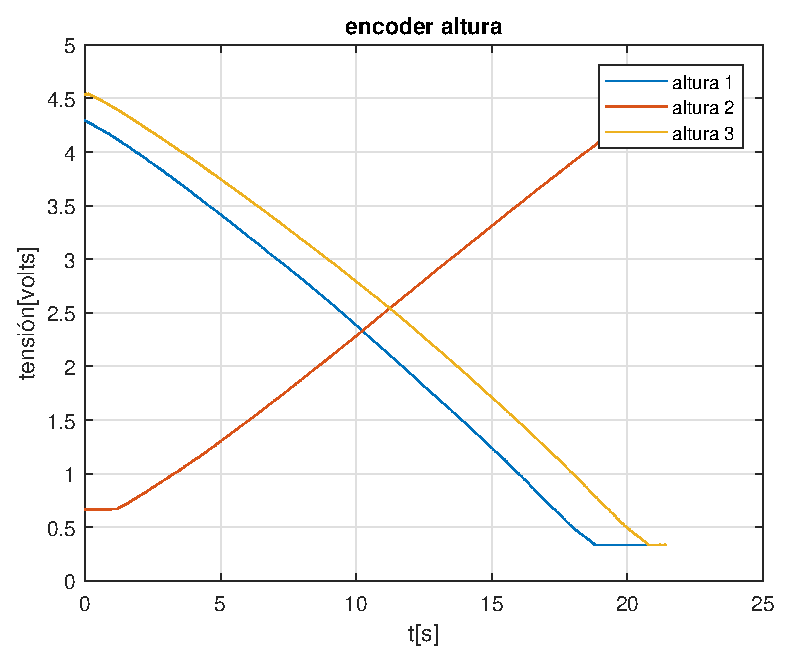
\includegraphics[width=\textwidth,height=6cm]{medidas_cenit} 
		\caption{Encoder de altura} 
		\label{subfig:altura} 
	\end{subfigure}
	\hspace{10mm}	
	\begin{subfigure}[t]{0.5\textwidth}
		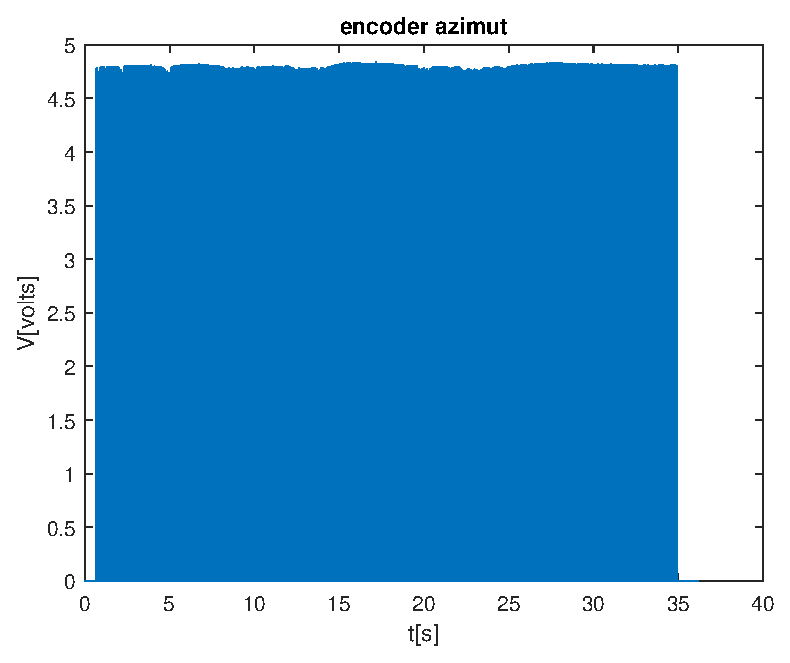
\includegraphics[width=\textwidth,height=6cm]{medidas_azimut}
		\caption{Encoder azimut}  
		\label{subfig:azimut} 
	\end{subfigure}
	\caption{Medidas realizadas sobre los encoders de la antena en función del tiempo.}
\end{figure}


Se observa en el ángulo de altura (ver figura \ref{subfig:altura}), que el potenciómetro responde de forma lineal en función del tiempo, mientras que el ángulo de azimut, utiliza una serie de pulsos para medir la posición angular (ver figura  \ref{subfig:azimut}). Este último, será reemplazado por un potenciómetro comercial en la fase 4. Esté, será de tipo lineal. 

De la función de autocalibración, obtenemos los valores máximos y mínimos del conversor A/D sobre el eje de altura, e idem cuando se adicione el potenciómetro en el eje de azimut. A partir de estos puntos, obtenemos la relación entre la tensión leída y los ángulos. Es decir, obtenemos una relación lineal entre la tensión del potenciómetro y el ángulo de la antena. En el microcontrolador, se usan los valores leídos del conversor analógico digital, para la programación.

Dado que el potenciómetro es lineal, puede construirse la ecuación de una recta, a partir de dos puntos. Estos dos puntos, son los valores máximos y mínimos del conversor A/D, y los ángulos máximos y mínimos de la antena. La convención utilizada para los ángulos se encuentra en la tabla \ref{tab:def_sist_coord}. Para el ángulo de azimut, se tienen los puntos 
\[ 
\begin{split}
p_1 &=(0^\circ,\min\{calibracion\_encoders[0],calibracion\_encoders[1]\}) \\
p_2&=(180^\circ,\max\{calibracion\_encoders[0],calibracion\_encoders[1]\})
\end{split}   
\]
 Al tener dos puntos, se puede armar la ecuación de una recta, en términos de $\theta_{az} = f(AD_0)$, siendo $\theta_{az}$ el ángulo de azimut. La ecuación de la recta, viene dada por:  

\begin{equation}
	\theta_{az} = \frac{\Delta \theta_{az}}{\Delta A_d}(AD_0 - \min\{  \text{calibracion\_encoders}[0],\text{calibracion\_encoders}[1]\}) 
\end{equation}
Siendo: 
\vspace{-2mm}
\begin{flalign*}
	& AD_0:\text{Valor leido por el conversor Analogico digital del puerto 0} &  \\
	&\Delta\theta_{az} = 180^\circ - 0^\circ & \\
	&y_1 =\min\{calibracion\_encoders[0],calibracion\_encoders[1]\}& \\ &y_2 =\max\{calibracion\_encoders[0],calibracion\_encoders[1]\} & \\
	&\Delta A_d = y_2 - y_1 & 
\end{flalign*}


Para el eje de altura, se realiza un procedimiento similar al anterior, se obtiene la ecuación de la altura en función del valor leído de tensión. Denominando $\theta_h$ al ángulo de altura,se obtiene la siguiente ecuación  

\begin{equation}
	\theta_h = \frac{\Delta \theta_h}{\Delta A_d}(AD_1 - \max\{  \text{calibracion\_encoders}[0],\text{calibracion\_encoders}[1]\}) 
\end{equation}
Siendo: 
\vspace{-2mm}
\begin{flalign*}
	& AD_1:\text{Valor leido por el conversor Analogico digital del puerto 1} &  \\
	&\Delta\theta_h = 90^\circ - 0^\circ & \\
	&y_1 =\max\{calibracion\_encoders[0],calibracion\_encoders[1]\}& \\ &y_2 =\min\{calibracion\_encoders[0],calibracion\_encoders[1]\} & \\
	&\Delta A_d = y_2 - y_1 & 
\end{flalign*}

Las ecuaciones mostradas anteriormente, se implementan dentro de la función \mintinline{Arduino}{leer_encoders.} 

Además de esto, se debe calcular la resolución angular del dispositivo para cada eje. Esta viene dada por las pendientes de las rectas anteriores, multiplicadas por 1, ya que es el mínimo valor de cuenta que posee el conversor analógico digital. Las resoluciones, son entonces: 
\begin{equation}
	\begin{split}
		res_h &= \frac{ \Delta\theta_h}{\Delta A_d}  1 = \frac{ \Delta\theta_h}{\Delta A_d} \\  
		res_{az} &= \frac{ \Delta\theta_h}{\Delta A_d}  1 = \frac{ \Delta\theta_h}{\Delta A_d}   	
	\end{split}
\end{equation}

Cabe destacar, qué como magnitud del error, se ha utilizado la resolución, para realizar pruebas. En realidad, se debe tener en cuenta el ángulo sólido de la antena para realizar el control. Esta discusión, sobre el ángulo sólido de una antena parabólica, rebasa el alcance del presente trabajo.
El esquema de control se muestra en la figura  \ref{fig:sist_control_real}. 

En esta parte, se programa el recuadro de la parte ``control\_motores(ref1,ref2)'' de la figura \ref{fig:sist_control_real}. El control, mira una señal de error, donde la señal de error en la figura viene dada por $e[k]$. Hay dos señales de error, estas las denominados $e_1 $ y $e_2$ .Estas señales de error vienen dadas por: 
\begin{equation}
	\begin{split}
		e_1[k]&=ref_1 - \text{azimut}  \\
	    e_2[k]&=ref_2 - \text{altura}  
	\end{split}
\end{equation}

\begin{figure}[pt]
	\hspace{-30mm}
	\includegraphics{control_realimentado}
	\caption{Sistema de control microcontrolado implementado en este trabajo.}
	\label{fig:sist_control_real}
\end{figure}

 En base a esta señal de error, que es entrada para el bloque ``control ON/OFF'', decide hacia donde debe moverse el motor. El sistema se para siempre que la señal de error sea menor que la resolución de cada eje. Este sistema en próximas versiones, se va a cambiar el bloque ``controlONOFF'' por un controlador denominado PID. 
\vspace{15mm}

 El control ON/OFF, actúa según la siguiente tabla, donde para seleccionar el sentido, se basa en las variables movimiento\_motor\_1 y movimiento\_motor\_2, que se obtienen de la función de autocalibración. 
 
 \begin{table}[ht]
 	\centering 
 	\begin{tabular}{|c|c|c|c|}
 		\hline 
 		eje & error & sentido de movimiento & valor variable sentido \\ 
 		\hline	 
 	%	\cline{3-4} 
 		\multirow{3}{*}{Azimut}& $e<-res_{az}$ & este$\rightarrow$ oeste  &movimiento\_motor\_1[1] \\ \cline{2-4}
 		& $e>res_{az}$& oeste$\rightarrow$ este& movimiento\_motor\_1[0] \\ \cline{2-4}
 	%	\hline
 		& $|e|<res_{az}$& motor parado & 0\\ \cline{2-4}
 		\hline   
 		\multirow{3}{*}{altura}& $e<-res_h $ &90° $\rightarrow$ plano del suelo& movimiento\_motor\_2[1] \\ \cline{2-4}
 		& $e>res_h$ &plano del suelo $\rightarrow$ 90° & movimiento\_motor\_2[0] \\ \cline{2-4}
 		& $|e|<res_h$& motor parado& 0\\ 
 		\hline
% 		\cline{2-4}
 		  			
  	\end{tabular}
 \end{table}  
 
La medida angular sobre la que se debe realizar el contron ON/OFF, se debe basar en el ángulo sólido de la antena, y en la potencia de ruido recibida por el microcontrolador (mas específicamente, la relación SNR, la explicación de esta, rebasa el alcance del presente informe). Esta potencia, nos da un indicativo de cual debe ser el intervalo del error para realizar el frenado de los motores en esa posición. Ambas medidas, no se pueden realizar, ya que el ángulo sólido de la antena, depende de la frecuencia de operación del receptor, mientras la potencia de ruido, depende del ambiente en el cual se coloque el dispositivo.   
 
% El valor para que se pueda realizar el control correctamente, debe medirse el ruido sobre el sistema(más específicamente, la potencia del ruido),y luego proponer un valor mayor a él para realizar el control, en lugar de la resolución. Se va a probar, si la antena, responde con este valor de resolución, o debe reajustarse. Además, se tomará en cuenta el ángulo solido de la antena parabólica. El código realizado para el control, se encuentra en el apéndice del presente texto. 

\subsection{Resultados de la función de autocalibración y control}

La función de control, requiere de la definición de los datos brindados por la función de autocalibración. Para la función de autocalibración, en la tabla \ref{tab:result_control} definimos los sentidos, siendo los resultados de las variables los que se encuentran en tabla \ref{tab:resultados_autocalibracion}. Luego, en base a estas variables, se observan cuales puertos son los correspondientes en base a los diodos leds referidos en la figura \ref{fig:proto_1}. La resolución, se definió en la sección anterior. El valor de referencia utilizado para realizar las pruebas es el denominado cenit: 90° en altura y 90° en azimut. 

En la tabla \ref{tab:result_control}, se observa que, la función de control responde como se esperaba, ya qué se observa que al cambiar el puntos inicial, para el mismo error, se invierte la dirección de los puertos. Esto es así, ya que la función de autocalibración, guarda el sentido de movimiento de la antena, y la función de control, los orienta en el sentido correcto.    


\begin{table}[ht]
%	\hspace{-25mm}
\resizebox{\linewidth}{!}
{
  \begin{threeparttable}		
	\begin{tabular}{|p{1.5cm}|p{1.5cm}|p{1.5cm}|c|c|c|c|c|c|}
		\hline 
		\multicolumn{9}{|c|}{Motor 1: Motor de azimut - Referencia 90º } \\
		\hline 
		\multicolumn{3}{|c|}{autocalibración} & \multicolumn{6}{c|}{control } \\
		\hline 
		\multirow{2}{1.4cm}{Posición inicial} &\multirow{2}{1.4cm}{ Primer Giro} & \multirow{2}{1.4cm}{Segundo giro} &\multicolumn{2}{c|}{$e>res_{az}$} &\multicolumn{2}{c|}{$e<-res_{az}$} &\multicolumn{2}{c|}{$|e|\leq res_{az}$} \\ \cline{4-9}
		
		 & &  & puerto on & puerto off &puerto on & puerto off&puerto off & puerto off\\ 
		\hline 
		punto medio & giro izquierda & giro derecha & MOTOR\_1\_S2 & MOTOR\_1\_S1  & MOTOR\_1\_S1& MOTOR\_1\_S2& MOTOR\_1\_S1 & MOTOR\_1\_S2 \\ 
		\hline 
		punto medio & giro derecha & giro izquierda &MOTOR\_1\_S1  &MOTOR\_1\_S2
		& MOTOR\_1\_S2&  MOTOR\_1\_S1 &MOTOR\_1\_S1 & MOTOR\_1\_S2 	\\
		\hline 
		extremo izquierdo & giro derecha & x &MOTOR\_1\_S2  & MOTOR\_1\_S1  & MOTOR\_1\_S1& MOTOR\_1\_S2 &MOTOR\_1\_S1 & MOTOR\_1\_S2 \\ 
		\hline 
		extremo derecho & giro izquierda & x & MOTOR\_1\_S1&MOTOR\_1\_S2  & MOTOR\_1\_S2 &MOTOR\_1\_S1 &MOTOR\_1\_S1 &MOTOR\_1\_S1  \\ 
		\hline 
		%---------------------------- MOTOR DE ALTURA 	--------------------------%
		\hline 
		\multicolumn{9}{|c|}{Motor 2: Motor de altura - Referencia 90º } \\
		\hline 
		\multicolumn{3}{|c|}{autocalibración} & \multicolumn{6}{c|}{control } \\
		\hline 
		\multirow{2}{1.4cm}{Posición inicial} &\multirow{2}{1.4cm}{ Primer Giro} & \multirow{2}{1.4cm}{Segundo giro} &\multicolumn{2}{c|}{$e>res_h$} & \multicolumn{2}{c|}{$e<-res_h$\tnote{1}}  &\multicolumn{2}{c|}{$|e|\leq res_h$} \\ \cline{4-9}
		
		& &  & puerto on & puerto off &puerto on & puerto off&puerto on & puerto off\\ 
		\hline 
		punto medio & giro izquierda & giro derecha &  MOTOR\_2\_S1 &  MOTOR\_2\_S2  & x & x &MOTOR\_2\_S1 &MOTOR\_2\_S2 \\ 
		\hline 
		punto medio & giro derecha & giro izquierda & MOTOR\_2\_S2 & MOTOR\_2\_S1 & x & x & LOW &LOW \\ 
		\hline  
		extremo izquierdo & giro derecha &x & MOTOR\_2\_S1 & MOTOR\_2\_S2  &   x  & x  &MOTOR\_2\_S1 &MOTOR\_2\_S2 \\ 
		\hline 
		extremo derecho & giro izquierda & x & MOTOR\_2\_S2 & MOTOR\_2\_S1  & x  & x  &MOTOR\_2\_S1 &MOTOR\_2\_S2 \\ 
		\hline 
	\end{tabular}
	\begin{tablenotes}
	 	\small 
	 	\item Los valores de los puertos en on y off,están definidas en el archivo ``pinout\_ard\_uno.h'', cuyo código se muestra en el código  \ref{cod:pinout_ard_uno.h}.
	 	
	 	\item [1] En el caso del motor de altura, al ser la referencia el máximo valor angular, el error, no puede darse que $e < -res_h $  
	\end{tablenotes}
	\end{threeparttable}
}	
	\caption{Resultados de la función de control en conjunto con la función de autocalibración.}
	\label{tab:result_control}
\end{table}


\section{Programación de Scheduler o planificador}

La programación por scheduler(o planifidor por su traducción al español), es la base del sistema operativo en tiempo real(p. ej FreeRtos\footnote{FreeRtos es un sistema operativo de tiempo real para sistemas embebidos}). El sistema consiste en la ejecución de tareas, que se denominan aplicaciones. Estas tareas, se ejecutan cada cierto tiempo, donde el tiempo lo define el programador. Esto puede definir tareas de mayor o menor prioridad, y permite la ejecución de tareas de forma asincrónica – sincrónica. La ejecución sincrónica, es la ejecución a tiempo controlado de la aplicación, mientras que la forma asincrónica, puede ejecutarse en cualquier parte del software. En este trabajo, se realiza, la programación de una base de tiempo para controlar la ejecución de tareas, y las funciones necesarias para controlar los relojes, definidos por el programador. Luego, se prueban estos relojes, con el uso de un osciloscopio, y midiendo los tiempos, y revisando que coincidan con el código desarrollado. 

\subsection{Funcionamiento base de tiempo para scheduler}

Este se basa en el concepto de interrupción. Las interrupciones se explican en el apéndice \ref{ap:ard_uno_env}. Se realiza una interrupción por timer es una interrupción sincrónica, definida por el programador. En el caso del Atmel ATMEGA 328P, posee tres timer, en el presente trabajo, se utiliza el timer2. El diagrama de este se muestra en la figura \ref{fig:timer_2}. 

\begin{figure}[ht]
	\includegraphics{timer_2}
	\caption{Diagrama del timer 2 }
	\label{fig:timer_2}
\end{figure}


Esta frecuencia se selecciona del clock principal, y se hace pasar por un divisor de frecuencia, llamado preescaler. Este preescaler, solo realiza divisiones de frecuencia en potencias de dos, y se configura con un registro llamado ``TCCR2B'', que además configura otros parámetros. Una vez configurada la frecuencia de las interrupciones, contamos cuantas interrupciones ocurren, y se tiene el tiempo para cada tarea. 

Este timer tiene 4 modos de funcionamiento. Los cuales son:  

\begin{itemize}
	\item NORMAL MODE 
	\item Clear Timer on Compare Match (CTC) Mode
	\item Fast PWM Mode 
	\item Phase Correct PWM Mode
\end{itemize}

Sin entrar en los detalles de cada uno de ellos, explicados en la hoja de datos del microcontrolador Atmel Atmega328P (\cite{ATmega328P}), los últimos dos modos, se usan para realizar un PWM, y el primero, cuenta hasta una cantidad fija, definida en 255. El modo elegido para este propósito fue el CTC (explicado en la siguiente sección), de todos los modos, es el que mejor se ajusta a una base de tiempo controlada. 


\subsection{Clear Timer on Compare Match (CTC) Mode }

Para configurar este modo, se deben configurar algunos registros, mostrados en la figura \ref{fig:timer_2}. En ella, se ve que los registros, tienen la terminación ``nx''. Esta terminación corresponde al número de timer y al canal. Así, n puede tomar el valor 0,1 o 2, y x la letra A o B. Por ejemplo: el registro OCR2A, corresponde al timer 2, y al canal A del mismo (\cite{ATmega328P}). 
 
El registro TCNT2, se incrementa de a uno, con la frecuencia de preescaler seleccionada en el registro TCCR2B. Cuando el valor de TCNT2 coincide con el valor cargado en el registro OCR2A, se lanza una interrupción por timer. El siguiente esquema aclara lo anterior. 

\begin{figure}[ht]
	\includegraphics{ctc_t2} 
	\caption{Diagrama de tiempos del modo CTC. Extraído de la hoja de datos del microcontrolador}
	\label{fig:ctc_isr}
\end{figure}

En el se ve, que la interrupción se ejecuta cuando TCNT2 alcanza a OCR2A. Para el cálculo de la frecuencia, usamos la siguiente formula, que viene dada por el fabricante del dispositivo
\begin{equation} \label{eq:frec_clk_isr2}
	f_{OCnx} = \frac{f_{clk \_ I/O}}{2N(1+OCRnx)}
\end{equation}
donde 

\begin{flalign}
	&f_{OCnx} : \text{frecuencia de el modo CTC.} & \\
	&N : \text{valor del preescaler,son algunas potencias de dos.} & 
	\\
	&f_{clk \_ I/0} : \text{frecuencia del reloj utilizado por el microcontrolador.} & 		
\end{flalign}

Esta ecuación para calcular la frecuencia, es la frecuencia de una onda cuadrada, en el caso de la imagen \ref{fig:ctc_isr}, es el periodo enumerado con ``1'', en la imagen. Por este motivo, para conocer la frecuencia de la interrupción, se debe multiplicar por dos, al valor que brinda esta ecuación. 


El valor de $f_{clk \_ I/0}$ es 16 Mhz, que es la frecuencia de reloj utilizada por la placa Arduino UNO (véase \cite{arduno}). En este caso, buscamos que el valor sea entero, o múltiplo de 10. Para realizar esto, se utilizaron varias pruebas. Se concluyeron los siguientes valores
\begin{itemize}
	\item N = 32
	\item OCR2A = 49
\end{itemize}

Si reemplazamos en la ecuación \ref{eq:frec_clk_isr2} nos brinda un valor de 5Khz. Entonces, la interrupción ocurrirá, con una frecuencia de 10Khz, o cada 100 $\mu$s. 

Para configurar el valor de N(denominado preescaler, dentro de la hoja de datos del microcontrolador), y la configuración CTC, dentro de cada timer, existen dos registros de configuración. 
Estos se llaman TCCR2A y TCCR2B, y 
Estos registros se deben configurar con los siguientes valores binarios: 
\begin{itemize}
	\item \textbf{TCCR2A = 0b00000010} 
	\item \textbf{TCCR2B = 0b00000011} 
\end{itemize} 

El valor de cada bit, esta detallado en la hoja de datos del microcontrolador (véase \cite{ATmega328P}), y no se van a explicar en el presente documento. Al final de realizar todo este análisis, se construyó una función, que automatice esta tarea de configuración. La función tiene por nombre \mintinline{Arduino}{Base_tiempo()}. El código se muestra a continuación. 

\begin{listing}[ht]
	\begin{minted}[linenos,frame=single]{Arduino}
void Base_tiempo()
{
 SREG = (SREG & 0b01111111);
 TCNT2 = 0 ;
 TIMSK2 = TIMSK2 | 0b00000010 ;
 TCCR2A = 0b00000010;
 TCCR2B = 0b00000011; // 0.5 MhZ n= 32 
 OCR2A = 49;
 SREG = (SREG & 0b01111111) | 0b10000000 ;
}	
	\end{minted}
\caption{Función base de tiempo.}
\label{cod:base_tiempo}
\end{listing}

Esta función, además de configurar el modo CTC, el preescalador , y el registro OCR2A, configura las interrupciones. La configuración de las interrupciones puede obtenerse de la hoja de datos del microcontrolador.

\subsection{Programación del Software scheduler} 

El software esta compuesto por 8 relojes, cuya cantidad puede programarse a partir del archivo ``tiempo.cpp'', el cual tiene una bandera denominada \mintinline{Arduino}{RELOJES}, para configurarse la cantidad de relojes deseada. 
Primero deben crearse los relojes, que pueden o no estar configurados. Estos relojes, los definimos como una matriz de 8x4, donde cada fila es el número de reloj, y cada columna es hora, minuto, segundo y milisegundo. Esta matriz se llama timer dentro del código. Luego, deben crearse las funciones para interactuar con ella, además,  debe crearse una bandera, que diga, que reloj o relojes contaron el tiempo preestablecido por el programador. Esto se logra con un vector de eventos, donde va guardando los relojes que han agotado su tiempo. Se usa un vector, porque puede qué exista más de un reloj que se agote su tiempo. Este vector se denomina FlagRepEvent[] dentro del código de programación. Además, creamos un vector que indica cuales relojes están activos, y lo llamamos timer\_activo. Todas estas variables, necesitan, comunicarse entre sí, y la comunicación entre ellas se realiza usando funciones. En la figura \ref{fig:soft_sch} se muestra un diagrama del software programado.  


\begin{figure}[ht]
	\includegraphics[width=\linewidth]{software_timer} 
	\caption{Diagrama de software para el software de scheduler}
	\label{fig:soft_sch} 	
\end{figure}

\subsubsection{Funciones}
Los archivos tiempo.cpp y .h ofrecen las siguientes funciones, encapsuladas en una librería:
\begin{itemize}
\item TimerStart(char n\_reloj,char h, char m, char s , int ms)
\item AnalizoTimer(char n\_reloj, char\_index) 
\item timerClose(char n\_reloj) 
\item timerStop(char n\_reloj)
\item timer\_marcha(char n\_reloj) 
\end{itemize}



\textbf{TimerStart}:  inicializa el número de reloj, con la cantidad de tiempo que desea el programador que se ejecute la tarea. Esta función carga la variable timer[n\_reloj][] con los valores de hora, minuto, segundo y milisegundo que desea el programador(es decir, carga la fila), y además carga el vector timer\_activo[] con el valor de reloj. 

\textbf{AnalizoTimer}: Esta función se ejecuta dentro de la interrupción. Su finalidad es descontar un milisegundo a los relojes que previamente se habían cargado. Esta lo que realiza, es solamente el decremento de un milisegundo en los relojes que estén activos en el flag timer\_activo. La función decrementa igual que lo haría un cronometro de bolsillo. Es decir, llega ms a cero, y mira los segundos, si los segundos no son cero, decrementa en uno el segundo, y pone en 999 la variable de ms en el número de reloj correspondiente.  

\textbf{TimerClose}: Esta función apaga el timer correspondiente, modificando el timer\_activo(poniéndolo a cero) y poniendo todo el reloj a cero. 

\textbf{TimerStop}: Deja de contar, es equivalente a parar un cronometro, para luego seguir contando. Esta función modifica timer\_activo y lo pone en cero, pero no modifica el vector de relojes, los cuales siguen sin ser modificados. Para volver a arrancar, se debe utilizar la función timer\_marcha, que vuelve a poner el funcionamiento el reloj que se había frenado. 

\textbf{timerEvent()}: esta función, observa la variable flagRepEvent[], y realiza la acción correspondiente, a ese tiempo asignado. En esta función, se asignan las tareas que debe realizar la planificación o scheduler.

\subsubsection{Funcionamiento del software} 

Este software se basa en el concepto de interrupción. Se genera una interrupción cada 100us, y con una variable se cuentan 10 de ellas, y ahí ha transcurrido 1ms. Luego de 10 interrupciones, se llama a la función AnalizoTimer(), que descuenta en un milisegundo de los relojes que estén activos, y si luego de descontar, todo el reloj es cero,(es decir, la fila n\_reloj es toda cero), activa el flagRepEvent correspondiente, para ejecutar la acción correspondiente. Esta acción, es activada por el switch -case de timerEvent() y ejecuta la aplicación correspondiente. 

El modo de utilizarlo es llamar a la función Base\_tiempo(), dentro del inicio del programa, luego con esto, se activan las interrupciones por timer. Acto seguido a esto, hay que definir el número de reloj a activar con la función TimerStart, o cuando se desee llamar, para activar el reloj correspondiente. Luego, debe definirse la acción a ejecutar por ese reloj, la cual debe estar definida dentro de la función timerEvent. 

Todo el código desarrollado para estas funciones, se halla en el CD que acopaña al presente documento.



\subsection{Resultados del software de planificación}

Luego de haber construido todo el software, se realizan dos pruebas, prendiendo y apagando dos leds, cada determinada cantidad de tiempo, y se ha utilizado un osciloscopio para ver la forma de onda.
 
En la primera prueba, se configuran dos relojes de 872ms, y se miden con un osciloscopio. Ambos se lanzan a tiempos distintos, es decir, existe un retardo entre ambos. Los resultados se midieron en el osciloscopio. La segunda prueba, fue configurar dos relojes, parar uno y relanzarlo, mientras el otro permanecía encendido. Los resultados de ambas pruebas sobre el osciloscopio se observan en las siguientes imágenes: 


\begin{figure}[ht]
%	\hspace{-20mm}
	\begin{subfigure}{0.5\linewidth}
		\centering
		\includegraphics[width=\linewidth]{osciloscopio_im1} 
		\caption{Primera prueba realizada sobre el software de scheduler}
		\label{fig:osc_m1}	
	\end{subfigure}
	\hfill
%	\hspace{20mm} 
	\begin{subfigure}{0.5\linewidth}
		\centering
		\includegraphics[width=\linewidth]{osciloscopio_im2}
		\caption{Segunda prueba realizada sobre el software de scheduler} 
		\label{fig:osc_m2}		
	\end{subfigure}
	\caption{prueba sobre el software de manejo de scheduler}
\end{figure}

Los códigos utilizados para medir esta función, no se encuentran dentro de este documento. Este, debe realizarse utilizando las funciones anteriores, y para la segunda prueba, poner un contador y parar el segundo reloj cuando llegue a un determinado valor, y seguir contando, y cuando alcance un segundo valor, volver a lanzar el mismo reloj. 

Como observamos, en la primera prueba, fue generar una onda cuadrada, donde el estado de alto era de 872ms, y bajo de ese mismo tiempo. En la figura \ref{fig:osc_m1}, se observa la forma de onda en alto, y puede verse qué con los cursores del osciloscopio, la medida, fue del mismo tiempo. 

% observaciones imagenes oscioloscopio % 

La segunda prueba, se observa en la imagen \ref{fig:osc_m2}, donde, se ha parado un reloj, durante un tiempo, y se ha vuelto a empezar, manteniendo una onda cuadrada sobre el otro puerto. El resultado fue satisfactorio, ya que se observa, en el osciloscopio, como se ha frenado un puerto, mientras el otro sigue funcionando, y al cabo de un tiempo, volvió a empezar.  
 

\section{Conexión del software con Gpredict y Stellarium} 

En esta sección, se muestran los componentes principales del software desarrollado para comunicarse con estos programas, y como obtener la posición hacia donde debe ir la antena. En la figura \ref{fig:sist_control_real}, se observa un recuadro, que dice ``decidir referencia''. En esta parte del desarrollo, se trata de ver como el software, decide esa referencia. Las referencias provienen de tres fuentes posibles: 
\begin{itemize}
	\item Gpredict.  
	\item Stellarium. 
	\item cenit(ningún software conectado).
\end{itemize} 

Para ello, dentro del programa principal, se crean dos variables: denominadas \mintinline{Arduino}{ref1} y \mintinline{Arduino}{ref2} respectivamente. Estas tendrán por defecto el valor del cenit (90° en ángulo de azimut y 90° en altura). Cuando existe una conexión, con alguno de estos programas, estos valores cambian automáticamente a aquellas coordenadas enviadas por algunos de los programas. Una vez finalizada la conexión con alguno de estos programas, estas vuelven a su valor inicial(posición del cenit). 

Antes de empezar a realizar el software para comunicarnos con ambos programas, debe obtenerse la dirección IP, qué en esta etapa, será asignada por DHCP. Luego, cuando se conecte a la red institucional, se le asignará una dirección ip fija, dada por el administrador de la red. 

\subsection{Conexión a la red mediante DHCP} 

En primer lugar, se debe conectar el chip ethernet w5100, mediante un cable denominado utp, a un switch o router.   Este cable es comúnmente conocido como cable de red.

 Una vez, el chip ethernet, se ha conectado físicamente a la red, mediante un cable de red, se deben obtener los parámetros de la red, mediante el uso del servicio de DHCP(por el momento,en un futuro será fija la dirección IP del dispositivo). El entorno Arduino, provee una librería para trabajar sobre el chip ethernet W5100. Esta librería, se denomina ``ethernet.h'', y viene por defecto en su entorno. Esta librería, se provee de varias funciones, para poder realizar la conexión con el chip W5100 y obtener la dirección IP mediante el protocolo DHCP. 
 
 Para comenzar a utilizar esta librería, en primer lugar, se debe armar la conexión como muestra la figura \ref{fig:esq_completo}. Una vez armado, se debe conectar el cable de red a la placa que posee el chip W5100. Una vez realizado, se debe realizar la petición DHCP mediante el uso de la librería. 

En primera instancia, debe realizarse la configuración del puerto de slave select. Esto se realiza con la sentencia:  

\mint{Arduino}|Ethernet.init(PINSS)| 

Una vez definido el pin de chip select, se debe asociar una dirección al dispositivo, denominada ``dirección mac''. Esta dirección es un identificador que está asociada a cada hardware que desee conectarse a la red. En el caso del chip w5100, esta dirección, se la debe dar el programador, ya que se configura mediante software. La manera de definir una dirección es: 

\mint{Arduino}|  byte mac [] = {0x00, 0xCD, 0xEF, 0xEE, 0xAA, 0xBC};|  

Ahora, debe procederse a obtener la dirección IP por DHCP. Las sentencias para obtener la dirección ip se muestran en el código \ref{cod:dhcpIP}. La dirección IP, que se le asigna mediante el protocolo DHCP, se muestra en el puerto serie, con este código.

\begin{listing}[ht]
	\begin{minted}[linenos,frame=single]{Arduino}
 if (Ethernet.begin(mac) == 0)
{
	Serial.print("obt_Ip") ;
	Serial.print(F("Fallo DHCP"));
	
} else {
	Serial.print(Ethernet.localIP());
}		
	\end{minted}
\caption{Obtención de la dirección IP usando el protocolo DHCP} 	
\label{cod:dhcpIP} 
\end{listing}


Una vez, obtenidos todos los parámetros de la red, se deben configurar los programas, Gpredict, y Stellarium. La dirección IP que se obtuvo a partir de los pasos mencionados, fue la 192.168.0.150. Esta, es la que se va a utilizar para configurar los programas. 

\subsection{Configuración de Gpredict - Programación de la comunicación} 

En primer lugar, debe realizarse la configuración del software Gpredict, siguiendo los pasos que se muestran en la sección \ref{subs:conf_Gpredict}, en la figura \ref{fig:conf_rot_ip}. Antes de realizar la configuración sobre el software, se debe recordar, que Gpredict, toma el cero del eje azimutal, en el polo norte geográfico, y en sentido de las agujas del reloj, aumenta la cantidad de grados, hasta llegar a 360º. Por este motivo, la configuración de Gpredict en el eje azimutal, debe ser entre 90º(corresponde al este), y 270º(corresponde al
oeste geográfico). Dicho esto, se configura el rotador como muestra la siguiente figura: 
 
\begin{figure}[H]
	\centering 
	\includegraphics{conf_rotador_gpr}
	\caption{Imagen de la configuración del software Gpredict para la antena ubicada en sala de control del IAR. }
	\label{fig:conf_rot_sala_control}
\end{figure}
%
\subsubsection{Panel de control del rotador}
Si se procede a abrir el rotador recién creado, se observa la siguiente imagen(ver sección \ref{subs:conf_Gpredict}): 

\begin{figure}[ht]
	\includegraphics{rotador_select}
	\caption{Panel de control del rotador en Gpredict}
	\label{fig:panel_control_gpr}
\end{figure}

Observamos en la imagen, que se tienen los siguientes partes: 

\begin{itemize}	
	\item azimut: posee las coordenadas del rotador, que se envían mediante el protocolo TCP/IP. Si el rotador está conectado, en la parte read, aparece la posición del rotador.  
	\item elevación: ídem que azimut, salvo que en el eje de altura  
	\item target: Se selecciona el satélite que se desea seguir. Oprimiendo el botón track, se aplica la posición de azimut y elevación del satélite a seguir, tanto a azimut como a elevación 
	\item settings: Se selecciona el rotador, y en tolerance, indica la tolerancia entre el valor leído y el valor enviado por el rotador. Cycle, es para uso interno del programa, y no debe modificarse. El botón engage es para conectarse al rotador mediante la red.   
\end{itemize}


En la parte izquierda de la figura \ref{fig:panel_control_gpr}, se encuentra una gráfica en coordenadas polares. Los círculos concéntricos, indican el ángulo de altura, siendo el circulo exterior un ángulo de altura de 0º, y el centro de 90º. El ángulo desde el norte, en sentido de las agujas del reloj, indica el ángulo de azimut. Este ángulo es el que está representado en la ventana de azimut y elevación, con un círculo rojo. Por ejemplo, en la imagen de la figura \ref{fig:panel_control_gpr}, se observa, 180º azimut, y 45º elevación, y el círculo rojo, está marcado apuntando al sur, y aproximadamente en la mitad del radio del centro, hasta el circulo más grande. La imagen \ref{fig:polar_plot_expl} aclara la explicación dada. En la figura, se observa que hay un recuadro a rayas rojas, esto indica, la visibilidad de la antena instalada en sala de control en el IAR. 


\begin{figure}[ht]
	\centering
	\includegraphics[height=8cm]{polar_plot}
	\caption{Diagrama de gráfico polar en software Gpredict.} 
	\label{fig:polar_plot_expl}
\end{figure}

De la figura, se observa, qué en el ángulo de azimut, se tiene un desfase de 270º, entre la convención de gpredict, y la convención utilizada en este trabajo. Por este motivo, a la coordenada recibida por el software Gpredict, debe restársele esta cantidad. Si denominamos $\theta_{azgpr}$ a la coordenada recibida por Gpredict, y $\theta_{az}$ a la coordenada que debe apuntarse, según nuestra convención, se tiene la siguiente ecuación:
\begin{equation}
	\theta_{az} =270^\circ - \theta_{azgpr}
\end{equation}

Por último, se observa en la sección target y settings, los botones engage y track. Su comportamiento, se describe en la tabla \ref{tab:track_eng_gpr}
%con la siguiente tabla: 

\begin{table}[h!]
	\begin{tabular}{|c|c|p{11.0cm}|}
		\hline 
		track & engaje & Descripción. \\
		\hline 
		off & off  & No se envían comandos al rotador y tampoco se lee su posición \\ 
		\hline 
		on  & off  &   La posición del controlador se actualizan con la posición destino pero no se envían comandos al rotador. La posición actual del rotador no se lee. Si el satélite objetivo esta fuera del alcance, las coordenadas del controlador se establecerán en donde se espera que aparezca el satélite. \\
		\hline 
		off & on  &   Las coordenadas azimut y altura, se envían al rotador, pero no se establece ningún satélite para seguir.  Este modo se puede usarse para controlar manualmente el rotador, o realizar una calibración de la antena. \\  
		\hline 
		on  & on   &La posición del satélite a seguir, se envía continuamente al rotador en caso de que exista un satélite dentro del campo de visión de la antena. Si el satélite no se encuentra dentro del campo de visión, se establece la ubicación de la antena para esperarlo, y luego seguirlo \\
		\hline 
				
	\end{tabular}
	\caption{comportamiento al oprimir los botones track y engage}
	\label{tab:track_eng_gpr}
\end{table}

De la tabla, se observa, que la comunicación mediante el protocolo TCP/IP, se debe oprimir el boton Engage. Si se oprime este botón, la coordenada enviada, será la que aparece en la parte del panel donde dice ``azimut y elevación''. Si se oprime ``track'', y luego ``engage'', la coordenada enviada por TCP/IP, será aquella en la cual, se encuentre el satélite seleccionado. 

\vspace{-2mm}
\subsection{Programación del microcontrolador} 

Después de configurar el programa Gpredict, para que realice la comunicación con el dispositivo desarrollado en el presente trabajo, utilizando la librería ``ethernet'', provista de manera nativa con el entorno de desarrollo arduino, se debe crear un objeto, denominado servidor. La sentencia, para crear este objeto es la siguiente: 

\begin{listing}[H]
	\begin{minted}[linenos,frame=single]{Arduino}
#define PORT_GPREDICT 4533 
EthernetServer Gpredict(PORT_GPREDICT)
	\end{minted}
\vspace{-10mm}
\caption{definición del objeto servidor dentro del entorno arduino}. 
\label{cod:obj_serv_gpr}
\end{listing}
\vspace{-5mm}
Donde se encuentra definido \mintinline{Arduino}{#define PORT_GPREDICT 4533}, es el puerto utilizado para la comunicación mediante el protocolo TCP/IP.

Luego, dentro del código principal, se debe realizar una captura de estos datos para poder manipularlos, y responder adecuadamente. Recordar que hay dos tipos de comandos, los comandos de tipo Get y de tipo Set. En la siguiente tabla, se ilustra el formato de los datos, tanto en la respuesta como en la llamada: 
%\setlength{\textheight}{240mm}
\begin{table}[H]
	\centering
	\vspace{-2mm}
 \begin{threeparttable}	
	\begin{tabular}{|p{3.0cm}|p{3.0cm}|p{3.5cm}|p{3.0cm}|} 
		\hline
		\multicolumn{2}{|c|}{Comandos tipo Get} &\multicolumn{2}{c|}{Comandos tipo Set}  
		\\ \hline 
		Protocolo de envio & respuesta & protocolo de envio & respuesta \\ \hline 
		comando\tnote{1} & par1$\backslash$npar2$\backslash$n & 
		comando\tnote{1} par1\tnote{2} par2\tnote{2}  $\backslash$n & par1$\backslash$npar2$\backslash$n  \\ 
		\hline 
	\end{tabular}
	\begin{tablenotes}
		\item [1] los comandos estan definidos en la tabla \ref{tab:commands_Gpredict}   
		\item [2] par1 y par2 son las coordenadas de azimut y elevación respectivamente.  
		
	\end{tablenotes}


\end{threeparttable}
	\caption{Envío de respuesta y comandos entre Gpredict y el microcontrolador.}
	\label{tab:protocol_tx_gpr}
\end{table}


Dentro de código principal, para saber si existe algún dispositivo que quiera conectarse, se debe realizar las siguientes sentencias: 

\begin{listing}[ht!]
	\begin{minted}[linenos,frame=single]{Arduino}
EthernetClient cliente_gpr = Gpredict.available() ;
if(cliente_gpr)
{

}
	\end{minted}
\vspace{-5mm}
\caption{captura de paquetes recibidos mediante el software Gpredict}
\label{cod:cliente_gpr}
\end{listing}

Dentro de las llaves debe ir la acción a realizar según el comando recibido. Los comandos que utiliza Gpredict, son los que se muestran en la tabla \ref{tab:commands_Gpredict}, y el formato para responder a estas peticiones, se encuentran en la tabla \ref{tab:protocol_tx_gpr}.
Para ejemplificar: suponga que se lee el valor de "P 155.20 38.3". Esto significa que la antena debe apuntar al punto 155.20° en azimut, y 38.3° en altura, pero  debe responder la petición, como indica la tabla \ref{tab:protocol_tx_gpr}. Si en vez de una P, llegase una ``p'', este comando, indica que debe responder su posición al programa. Supongamos que la antena, se encuentra en la posición 125.0° en azimut, y 39° en altura, la respuesta a esta petición será ``125.0\textbackslash n 39°\textbackslash n'', siendo ``\textbackslash n'' un carácter de salto de línea  y en la pantalla de Gpredict, aparecerán estas coordenadas. En este ejemplo, no se aplicó la corrección de las coordenadas, están implementadas dentro del software. En el caso, que llegue un comando q(desconectarse del gpredict),se debe cambiar la referencia al cenit. En caso de el comando S, se debe para la antena, mediante la función ``mover\_antena''. El código desarrollado, se encuentra en el CD anexo al presente informe.




\subsection{Stellarium}

Para el stellarium, debe configurarse el software, según la sección \ref{sub:conf_stellarium_red}. Una vez allí, se configura el software como muestra la siguiente figura 
%\ref{fig:conf_net_stell}. 

\begin{figure}[ht]
	\centering 
	\includegraphics[scale=0.5]{configuracion_telescopio}
	\caption{configuración del stellarium} 
	\label{fig:conf_net_stell}
\end{figure}  

Una vez configurado, debe presionar ``control + 0'' o en la barra inferior, debe buscar el icono que le diga ``mover el telescopio a las coordenadas definidas''. Una vez allí, se le abrirá una ventana con la opción de ``configurar telescopio''. Debe abrir esa ventana, y le aparecerá el telescopio configurado recientemente. Puede configurar más de un telescopio si así lo desea. Aparecerá una ventana como la que se muestra en la figura \ref{fig:rotador_stellarium_conn}. 
 

\begin{figure}[ht!]
	\centering
	\includegraphics[scale=0.6]{rotador_stellarium} 
	\caption{Apertura del telescopio recién creado.}
	\label{fig:rotador_stellarium_conn}
\end{figure}
Una vez, ahí dentro, presionando el botón conectar, se aprecia la siguiente ventana que aparece en la siguiente imagen: %\ref{control del telescopio en stellarium}.  

\begin{figure}[ht!]
	\includegraphics{rotar_telesc}
	\caption{Imagen del panel de control del telescopio usando Stellarium}
	\label{control del telescopio en stellarium}
\end{figure}
donde se observan los siguientes botones y opciones: 
\begin{itemize}
	\item Rotar: envía las coordenadas al dispositivo que mueve la antena, en el caso del presente documento, es el dispositivo desarrollado en este trabajo. 
	\item Sync: En desuso, no posee ningún tipo de uso. 
	\item Ascensión recta: tipo de coordenadas para visualizar estrellas. 
	\item declinación: ídem que ascensión recta.  
	\item objeto actual, centro de la pantalla: Permite poner las coordenadas en a donde debe apuntar el telescopio, usando algún astro seleccionado, o el centro de la pantalla. 
	\item HMS, GMS,DECIMAL: tipo de ángulo mostrado. HMS es utilizando el sistema de medición angular basado en horas, el segundo, es el sexagesimal, y el tercero es el decimal. 
\end{itemize}

Este software, no trae límites para el control de la antena, ya qué al ser un software utilizado para telescopios, supone que puede girar 360° en azimut y 90° en altura. El sistema de coordenadas utilizado se denomina ecuatorial, y debe realizarse una transformación de coordenadas para poder mover la antena. Esta transformación, se realiza en la siguiente fase del desarrollo del proyecto. 



\subsection{Programación para conectarse con Stellarium} 

En este caso, se debe definir un nuevo objeto servidor. La nueva definición del objeto se realiza de la siguiente manera: 

\begin{listing}[ht]
	\begin{minted}[linenos,frame=single]{Arduino}
#define PORT_STELLARIUM 10000
EthernetServer stelarium(PORT_STELLARIUM) ;      // socket tcp/ip para stelarium 
	\end{minted}
\caption{definición de objeto servidor para conectarse con el stellarium}
\end{listing}

En la sección \ref{sub:comun_stell}, se explica como envía los datos el stellarium, es decir, la trama de datos. En esta sección, se explica que el programa stellarium, llama a un software externo para enviar estos datos a través del protocolo TCP/IP. Este se denomina ``telescope\_server''. La codificación que utiliza, es la siguiente, dentro de los bits, la cual según su documentación(\cite{telscopeserv}), utiliza los ángulos en un sistema decimal (los siguientes datos estan en sistema hexadecimal): 

\begin{itemize}
	\item ascención recta: 
		\begin{itemize}
		 \item	ascensión recta 0hs  = 0x100000000   		
		 \item	ascensión recta 12hs = 0x80000000 
		 \item	ascensión recta 24hs = 0x00000000
	\end{itemize}
	\item declinación: 
		\begin{itemize}
		  \item	declinación -90° = -0x40000000
		  \item	declinación  0°  =  0x00000000
		  \item	declinación -90° = -0x40000000
		\end{itemize}
\end{itemize}

y con estos valores, se realiza una regla de tres simple, para ambos ejes coordenados. 

Dado que los bits, llegan desordenados(es decir, llegan en orden inverso), se los debe ordenar, para luego realizar la regla de tres simple, las instrucciones para organizar estos datos son: 

\begin{listing}[H]
%\hspace{-30mm}	
\begin{minted}[linenos,frame=single,breaklines]{Arduino}
uint8_t sunP[19] ; 
... 

dec = 0x00000000 | (long (sunP[19])<<24) | (long (sunP[18])<<16) | (long (sunP[17])<<8) | (long (sunP[16])<<0);
RA  = 0x00000000 | (long (sunP[15])<<24) | (long (sunP[14])<<16) | (long (sunP[13])<<8) | (long (sunP[12])<<0);
 	
\end{minted}
\caption{Reorganización de los datos recibidos desde el programa stellarium dentro del microcontrolador}
\label{cod:bitwise_order}
\end{listing}

Donde las variables dec y RA, son las coordenadas recibidas desde el software stellarium, los bits recibidos, se guardan en el vector uint8\_t sunP[20].

Una vez se realiza esto, se debe definir el código para que el microcontrolador, se comunique con el software stellarium. Este código, se realiza dentro del bucle principal del programa, y se le añade el código \label{cod:bitwise_order}, dentro del comportamiento. El código es el siguiente: 

\begin{listing}[ht!]
	\begin{minted}[frame=single,linenos,texcomments,escapeinside=||]{Arduino}
EthernetClient cliente_s = stellarium.available() ; 
long int dec ; 
unsigned long int RA = 0 ; 
uint8_t sunP[20] ; // vector datos recibidos 
char state_con = 0 ; 
if (cliente_s)
{
	
}
	\end{minted}
\caption{Parte del software que se encarga de conectarse con el software stellarium programado dentro del microcontrolador.}
\label{cod:connect_stellarium}
\end{listing} 

Luego, dentro de cada bloque if (ver código \ref{cod:cliente_gpr} y código \ref{cod:connect_stellarium}), van otras líneas adicionales, las cuales no se han mostrado para no extender el documento. Estas líneas adicionales se encuentran dentro del anexo del presente capítulo, y se encargan de mantener la conexión entre los programas de la PC, y el microcontrolador. 
   
\subsection{Resultados de la conexión con Gpredict y Stellarium} 

En esta sección, se comprueba la conexión, el intercambio de mensajes entre stellarium y Gpredict, con el microntrolador Atmega328p, utilizando como interface de red, el dispositivo el chip ethernet w5100. 

La herramienta seleccionada para realizar este análisis es el software WireShark, que se muestra en el capítulo de redes. Cada software se analiza por separado. Cabe mencionar, que el chip utilizado, no soporta ambos software trabajando en simultaneo, debido a sus limitaciones físicas, impuestas por el fabricante. Por este motivo, se prueban ambos programas por separado. 

\subsubsection{Conexión con Gpredict} 

Una vez, configurado el software Gpredict, para conectarse, se debe abrir el panel de control del rotador, y se debe oprimir el boton ``engage'' para calibrar la antena. Si la conexión funciona, dentro de los cuadros de azimut y elevación, se obtienen la posición de la antena (donde dice ``read'' en la figura \ref{fig:panel_control_gpr}). Esta posición, aparece como una cruz roja en el polar plot. El punto rojo, es la posición a la que se debe dirigir la antena, la cual es la coordenada azimut y altura, marcada con números más grandes en la imagen \ref{fig:panel_control_gpr}. 


\begin{figure}[ht]
	\includegraphics[scale=0.7]{gpred_rotador} 
	\caption{Conexión del microcontrolador al software Gpredict mediante el uso del protocolo TCP/IP} 
	\label{fig:prueba_gpredict_1} 
\end{figure}

En la prueba siguiente, se le dio a la antena, una altura de 45° y ángulo de azimut de 180°. Esta posición está marcada con un círculo rojo dentro de la gráfica polar. La posición que se encuentra el rotador, es de 253.78° en azimut y 47.85° en altura, esta posición se encuentra marcada con una cruz roja dentro de la gráfica polar(ver figura \ref{fig:prueba_gpredict_1}). A continuación, se han movido los potenciómetros manualmente,  y se nota que, al llegar a la posición, todos los leds del protoboard, permanecen apagados. Esto es un indicativo, que tanto el control como el software responden de manera apropiada. 

 
Luego de esta prueba, se ha probado el seguimiento de un satélite, de forma manual(es decir, moviendo los potenciómetros), en este caso, aparece el círculo rojo, la cruz indicando la posición de la antena, y un punto rojo, el cual indica la posición del satélite en el plano polar. Durante la prueba, se ha utilizado el software wireshark, para monitorizar los comandos enviados y recibidos desde Gpredict. En los comandos enviados y recibidos, no se ha mostrado ningún tipo de anomalía. En la figura \ref{fig:prueba_gpr_seg_sat} se dejan los resultados del panel de control  y en la figura \ref{fig:wireshark_gpr} los resultados del análisis hecho con wireshark. 


%A continuación, se dejan los resultados del panel de control

\begin{figure}[ht]
	\centering
	\includegraphics[scale=0.5]{gpredict_seguimiento_sat} 
	\caption{Panel de control del monitor realizando un seguimiento satelital} 
	\label{fig:prueba_gpr_seg_sat}	
\end{figure}

\begin{figure}[ht]
	\includegraphics[scale=0.5]{wireshark_gpredict} 
	\caption{Captura de paquetes TCP/IP utilizando el programa wirwshark mediante el seguimiento de un satelite} 
	\label{fig:wireshark_gpr}
\end{figure}



\subsubsection{Conexión con Stellarium} 

En el caso de stellarium, al no poseer un panel de control, como el Gpredict, se debe verificar de alguna forma, que las coordenadas recibidas, sean las correctas. En este caso, se usa el puerto serie como medio de depuración. Dentro del código, se transforman las coordenadas y se verifica que la unidad angular sea la correcta. Además, se realiza una verificación mediante el software wireshark para asegurarse que la comunicación sea fiable, y se respeten los protocolos entre ambos dispositivos(PC y microcontrolador).
Para verificar si las coordenadas son correctas, se ha oprimido el botón ``centro de la pantalla'', y luego el botón rotar. La figura \ref{fig:rotador_antena_stell_test} muestra las coordenadas enviadas por el panel de control del telescopio del software stellarium, y en la figura \ref{fig:coord_test_stell} se observan los resultados por puerto serie. 

Cabe destacar, que el ángulo de ascensión recta marcado por el stellarium es de -109,41°, y el del programa desarrollado, es de 250.58°. Este desfasaje, se da, por el signo negativo de la ascensión recta. Este signo negativo, indica que es contrario al sentido establecido por los astrónomos en este tipo de coordenadas. Para transformarla, se debe restarle 360° a ese ángulo, y se obtendrá la ascensión recta. La cuenta que debe realizarse es: 
\begin{equation*}
	360^\circ - 109.41^\circ = 250.58 
\end{equation*}

 Se observa, que el ángulo coincide, con el valor predicho, esto se observa en la imagen \ref{fig:coord_test_stell}.  
\begin{figure}[ht!]
	\includegraphics{rotador_antena_stell} 
	\caption{Panel de control del rotador del stellarium al momento de realizar las pruebas sobre el software} 
	\label{fig:rotador_antena_stell_test}
\end{figure}

\begin{figure}[ht!]
	\includegraphics{puerto_comm_stellarium}
	\caption{Coordenadas recibidas por el stellarium}
	\label{fig:coord_test_stell}
\end{figure}


Además, se revisa la conexión mediante el software wireshark. Los resultados del análisis se muestran en la imagen 	\ref{fig:wireshark_stell}.



\begin{figure}[ht!]
	\includegraphics[width=\linewidth]{wireshark_stellarium}
	\caption{Coordenadas recibidas por el stellarium}
	\label{fig:wireshark_stell}
\end{figure}

\section{Integración de partes del software} 

En esta sección se procede a unir todas las partes desarrolladas en esta etapa. Esta integración, se realiza utilizando el esquema de la figura \ref{fig:sistema_general}. La primera parte, debe realizar la función de autocalibración, luego debe iniciar el control de la antena, para volverla a su posición de equilibrio.  

Para realizar el control de la antena, se debe llamar a la función \mintinline{Arduino}{Leer_encoders()}, acto seguido, a la función de control, \mintinline{Arduino}{controlMotores(ref1, ref2)}. Esto debe realizarse periódicamente, por ende, dentro de la programación del scheduler deben ponerse ambas funciones. El tiempo de control seleccionado es 10ms. Estas funciones, se encuentran dentro del archivo ``timer.cpp''. Para inicializar dichas funciones, se debe realizar el código mostrado en la función setup, del archivo ``main.cpp'' mostrado en el apéndice del presente capítulo. Asimismo, en esta función, se programa, la obtención de la IP por DHCP, y se muestra por el display LCD. 

%\begin{listing}[ht]
%	\begin{minted}[linenos,frame=single,escapeinside=||]{Arduino}
%
%#define NUMBER_CLOCK 0 
%#define HOUR_CLOCK  0 
%#define MINUTE_CLOCK  0 
%#define SEGUNDO_CLOCK  0 
%#define MILISECOND_CLOCK  10 
%
%|   aqui siguien otras definiciones ... |
%...
%   |puesta en marcha del control cada 10 milisegundos |
%Base_tiempo() ; 
%timerStart(NUMBER_CLOCK,HOUR_CLOCK,MINUTE_CLOCK,SEGUNDO_CLOCK,MILISECOND_CLOCK)
%
%| en el bucle principal del programa debe ir |
%timerEvent() ; 
%
%	\end{minted}
%\caption{Inicialización del scheduler para leer los encoders y realizar el control de los motores.} 
%\label{cod:control_scheduler}
%\end{listing} 


%
%
%\begin{listing}[ht]
%	\begin{minted}[linenos,frame=single,escapeinside=||]{Arduino}
%void setup() 
%{
%	// debugger -- 
%	Serial.begin(9600) ; 
%	/**** inicializacion de puertos del motor como salida  *****/
%	init_pins_motores() ; 
%	autocalibracion()  ;
%	// inicializacion de ethernet 
%	Ethernet.init(PINSS) ; 
%	byte mac [] = {0x00, 0xCD, 0xEF, 0xEE, 0xAA, 0xBC}; // dirmac
%	#if ETHERNET_IP_LOCAL 
%	if (Ethernet.begin(mac,ip,DNS,gateway,mask_net) == 0)
%	{
%		Serial.print(F("Fallo DHCP"));    
%	}else 
%	{
%		Serial.print(Ethernet.localIP());
%	}
%	#else 
%	if (Ethernet.begin(mac) == 0)
%	{
%		Serial.print(F("Fallo DHCP"));    
%	}else 
%	{
%		Serial.print(Ethernet.localIP());
%	}
%	#endif
%	// inicio scheduler -- > 
%	Base_tiempo() ; 
%	timerStart(NUMBER_CLOCK,HOUR_CLOCK,MINUTE_CLOCK,SEGUNDO_CLOCK,MILISECOND_CLOCK) ; 
%	
%
%}
%
%void loop() 
%{
%	timerEvent() ; 
%	EthernetClient cliente_gpr = Gpredict.available() ;
%	EthernetClient cliente_s = stellarium.available() ; 
%	long int dec ; 
%	unsigned long int RA = 0 ; 
%	uint8_t sunP[20] ; // vector datos recibidos -- sunposition 
%	char state_con = 0 ; 
%	if(cliente_gpr)
%	{
%		
%	} 
%	if(cliente_s)
%	{
%		
%	} 
%	
%
%}		
%	\end{minted}
%\caption{código principal del proyecto.}
%\label{cod:main_cpp}
%\end{listing} 
%
La información angular, el número de IP, la depuración de variables, etc, se realiza mediante el puerto serie. En la próxima sección, se utiliza el display LCD para mostrar la dirección IP, y como se utilizan sus métodos para escribir texto en ella. Esto se realiza en el mismo reloj definido para utilizar la función leer\_encoders y controlMotores(ref1,ref2) ; 

\subsection{Resultados}
Para realizar la depuración del software realizado hasta este momento del desarrollo, se han realizado los siguientes pasos: 
\begin{enumerate}
	\item Se conecto Gpredict con el rotador. 
	\item Se movieron los potenciómetros, y se revisó que el ángulo de movimiento total de la antena sea el de la figura \ref{fig:panel_control_gpr}
	\item Se conecto Stellarium con el rotador.
	\item Se mueve la posición del software stellarium, y quedan registrados los datos por puerto serie.
\end{enumerate}


Luego de realizados estos pasos, se comprobó que todo el software respondía de forma correcta, y no se encontró ningún tipo de Bug o error en el código.

\section{Programación del display LCD} 

El entorno arduino, provee una librería específica para el manejo del display con el chip PCF8574. Esta se denomina \mintinline{Arduino}{LyquidCrystal_I2C}. Para utilizarla, se debe incluir en el archivo principal del proyecto. Una vez incluida, se debe crear un objeto LCD, que será el encargado de realizar todas las funciones del display. El objeto LCD se crea de la siguiente forma: 
\mintinline{Arduino}|LiquidCrystal_I2C lcd (ADRRESS_LCD_I2C,COLS_LCD,FILAS_LCD)|,
donde ADRESS\_LCD tiene el valor 0x27, que es la dirección del display para el uso del I2C(ver apéndice \ref{AP:protSerial}). 

Algunos de los métodos que posee esta clase, son: 
\begin{itemize}
	\item \mintinline{Arduino}{print(String c)}: imprime el String c en el display. 
	\item \mintinline{Arduino}{setCursor(x,y)}: posiciona el cursor en una fila y columna(x es la columna e y es la fila) 
	\item \mintinline{Arduino}{backlight()}:prende el backlight del display LCD.   
\end{itemize}

Estas funciones, serán utilizadas para mostrar información en el display LCD, reemplazando al puerto serie. En el código anexado al presente documento, ya se encuentra implementado. 



\section{Análisis del código realizado}

En esta sección, se muestran las principales métricas relacionadas al código. 
En primer lugar, se cuentan las líneas de desarrollo, utilizando la herramienta de visual Studio Code denominada VSCodeCounter. Los resultados se resumen a continuación: 

\begin{table}[ht]
	\centering
	\begin{tabular}{|c|c|c|c|c|c|}
		\hline 
		lenguaje& archivos & código & comentarios & lineas en blanco & total \\ 
		\hline 
		C++ & 8 &692 &189 &197 & 1078 \\
		\hline 
		ini &1 &13 &9 &2&24\\
		\hline
	\end{tabular}
	\caption{Tabla resumen de las líneas de desarrollo realizadas hasta el momento}
\end{table}
\vspace{-5mm}
Luego de esto, se analiza, los resultados arrojados por el compilador, que el código ocupa 80\% de la memoria de programa, y 52.9\% de la memoria RAM. 

Viendo la gran cantidad de memoria de programa que ocupa, se realizó un análisis con mayor profundidad del código, utilizando una herramienta de desarrollo conocida como ``avr-obj-dump''. La explicación de esta herramienta rebasa el alcance de este documento. Solamente se dirá que es una herramienta para analizar la memoria de microcontroladores AVR, revisando variables, objetos, etc. Una de las conclusiones, que se pueden obtener utilizando este método, es que las librerías de Arduino, se cargan de forma completa dentro del microcontrolador. No distingue entre funciones que usa y cuales no, el compilador. Debido a esta situación,  ha agregado código para aumentar la capacidad de la memoria FLASH. En la siguiente figura se deja una imagen con los resultados del obj dump.  

\begin{figure}[ht!]	
	\includegraphics[width=\linewidth,height=5.3cm]{dump_memory}
	\caption{Programa desensamblado en código assembler del microcontrolador. Se utilizó la herramienta avr-obj-dump. }
	\label{fig:avr_obj_dump}
\end{figure}


\section{Conclusiones}

En este capítulo, se muestra como han sido los pasos para construir un apuntador de antena basado en tecnología arduino, y sus librerías. Las librerías, poseen la desventaja de cargarse en memoria sin distinción acerca del uso o no de la funcionalidad. Esto, es un punto en contra, pero la velocidad de desarrollo mediante el uso de estas librerías, es superior si uno debe realizar los desarrollos desde cero.  

Se ha logrado realizar un control de tipo ON/Off, a pesar de las limitaciones del microcontrolador, y que respondan de manera adecuada a los requerimientos del proyecto, además, posee un manejo muy preciso de los tiempos de actuación, a pesar de ser un procesador de bajo costo en el mercado local. 


Para finalizar, esta sección, se ha construido la gran parte del software en esta sección, queda la parte de transformación de coordenadas, que será analizada y aplicada en la próxima fase. La construcción de esta función, requiere de conocimientos de trigonometría esférica, ya que todas estas coordenadas utilizadas, se refieren a una esfera. 

